%%%%%%%% ICML 2026 EXAMPLE LATEX SUBMISSION FILE %%%%%%%%%%%%%%%%%

\documentclass{article}

% Recommended, but optional, packages for figures and better typesetting:
\usepackage{microtype}
\usepackage{graphicx}
\usepackage{subcaption}
\usepackage{booktabs} % for professional tables

% hyperref makes hyperlinks in the resulting PDF.
% If your build breaks (sometimes temporarily if a hyperlink spans a page)
% please comment out the following usepackage line and replace
% \usepackage{icml2026} with \usepackage[nohyperref]{icml2026} above.
\usepackage{hyperref}

\usepackage{multirow}
\usepackage{bm}
\usepackage{colortbl}
\usepackage{xcolor}
\definecolor{grayhighlight}{gray}{0.9} % 定义浅灰色
% Attempt to make hyperref and algorithmic work together better:
\newcommand{\theHalgorithm}{\arabic{algorithm}}

% Use the following line for the initial blind version submitted for review:
\usepackage[preprint]{icml2026}
% 尝试清空预印本的文字变量（如果模板使用此变量）
\newcommand{\icmlpreprinttext}{}
\renewcommand{\icmlpreprinttext}{}
% For preprint, use
% \usepackage[preprint]{icml2026}

% If accepted, instead use the following line for the camera-ready submission:
% \usepackage[accepted]{icml2026}

\usepackage{amsmath}
\usepackage{amssymb}
\usepackage{mathtools}
\usepackage{amsthm}


% if you use cleveref..
\usepackage[capitalize,noabbrev]{cleveref}

%%%%%%%%%%%%%%%%%%%%%%%%%%%%%%%%
% THEOREMS
%%%%%%%%%%%%%%%%%%%%%%%%%%%%%%%%
\theoremstyle{plain}
\newtheorem{theorem}{Theorem}[section]
\newtheorem{proposition}[theorem]{Proposition}
\newtheorem{lemma}[theorem]{Lemma}
\newtheorem{corollary}[theorem]{Corollary}
\theoremstyle{definition}
\newtheorem{definition}[theorem]{Definition}
\newtheorem{assumption}[theorem]{Assumption}
\theoremstyle{remark}
\newtheorem{remark}[theorem]{Remark}

% Todonotes is useful during development; simply uncomment the next line
%    and comment out the line below the next line to turn off comments
%\usepackage[disable,textsize=tiny]{todonotes}
\usepackage[textsize=tiny]{todonotes}
\usepackage{bm}
% The \icmltitle you define below is probably too long as a header.
% Therefore, a short form for the running title is supplied here:
\icmltitlerunning{ Optimistic Distributionally Robust Policy Optimization for Off-Policy Generative Recommendation}
\setlength{\abovedisplayskip}{3pt}
\setlength{\belowdisplayskip}{3pt}

\usepackage[absolute,overlay]{textpos}

\usepackage{fancyhdr}
\pagestyle{fancy}

\begin{document}


\begin{textblock*}{\paperwidth}(1.5cm, 1.2cm)

\includegraphics[height=1.5cm]{figures/logo_v2.png} % 请确保目录下有 logo.png
\end{textblock*}

\twocolumn[
  \icmltitle{Breaking the Curse of Repulsion: Optimistic Distributionally Robust Policy Optimization for Off-Policy Generative Recommendation}

  % It is OKAY to include author information, even for blind submissions: the
  % style file will automatically remove it for you unless you've provided
  % the [accepted] option to the icml2026 package.

  % List of affiliations: The first argument should be a (short) identifier you
  % will use later to specify author affiliations Academic affiliations
  % should list Department, University, City, Region, Country Industry
  % affiliations should list Company, City, Region, Country

  % You can specify symbols, otherwise they are numbered in order. Ideally, you
  % should not use this facility. Affiliations will be numbered in order of
  % appearance and this is the preferred way.
  \icmlsetsymbol{equal}{*}

  \begin{icmlauthorlist}
    \icmlauthor{Jie Jiang}{equal,comp}
    \icmlauthor{Yusen Huo}{equal,comp}
    \icmlauthor{Xiangxin Zhan}{comp}
    \icmlauthor{Changping Wang}{comp}
    \icmlauthor{Jun Zhang}{comp}
  \end{icmlauthorlist}
  \icmlaffiliation{comp}{Tencent Inc, China}

  \icmlcorrespondingauthor{Jun Zhang}{neoxzhang@tencent.com}

  % You may provide any keywords that you find helpful for describing your
  % paper; these are used to populate the "keywords" metadata in the PDF but
  % will not be shown in the document
  \icmlkeywords{Reinforcement Learning, Recommendation System, DRPO}

  \vskip 0.3in
]

% this must go after the closing bracket ] following \twocolumn[ ...

% This command actually creates the footnote in the first column listing the
% affiliations and the copyright notice. The command takes one argument, which
% is text to display at the start of the footnote. The \icmlEqualContribution
% command is standard text for equal contribution. Remove it (just {}) if you
% do not need this facility.

% Use ONE of the following lines. DO NOT remove the command.
% If you have no special notice, KEEP empty braces:
% \printAffiliationsAndNotice{}  % no special notice (required even if empty)
% Or, if applicable, use the standard equal contribution text:

\printAffiliationsAndNotice{\icmlEqualContribution}


\begin{abstract}
 Policy-based Reinforcement Learning (RL) has established itself as the dominant paradigm in generative recommendation for optimizing sequential user interactions. However, when applied to offline historical logs, these methods suffer a critical failure: the dominance of low-quality data induces severe model collapse. We first establish the \textit{Divergence Theory of Repulsive Optimization}, revealing that negative gradient updates inherently trigger exponential intensity explosion during off-policy training. This theory elucidates the \textbf{inherent dilemma} of existing methods, exposing their inability to reconcile variance reduction and noise imitation. To break this curse, we argue that the solution lies in rigorously identifying the latent high-quality distribution entangled within the noisy behavior policy. Accordingly, we reformulate the objective as an \textbf{Optimistic Distributionally Robust Optimization (DRO)} problem. Guided by this formulation, we propose \textbf{D}istributionally \textbf{R}obust \textbf{P}olicy \textbf{O}ptimization (\textbf{DRPO}). We prove that hard filtering is the exact solution to this DRO objective, enabling DRPO to optimally recover high-quality behaviors while strictly discarding divergence-inducing noise. Extensive experiments demonstrate that DRPO achieves state-of-the-art performance on mixed-quality recommendation benchmarks.
 % while generalizing effectively to broader continuous control tasks.


\end{abstract}

\section{Introduction}
\label{sec:intro}

Generative recommendation has fundamentally transformed the field by reformulating recommendation as a sequential decision-making process\cite{geng2022recommendation, rajput2023recommender}. This approach maps user states directly to continuous item embeddings, creating a natural synergy with Reinforcement Learning (RL) frameworks like OneRec\cite{onerec}. However, applying RL in this context faces critical hurdles: the exponential action space and sparse rewards render efficient exploration prohibitively difficult\cite{dulac2015deep, chen2019top}, often trapping models in suboptimal local optima. To surmount these hurdles, we leverage the massive offline logs accumulated by traditional systems. By reconceptualizing this historical data as a rich repository for Offline (Off-policy) RL\cite{levine2020offline, fujimoto2019off}, we bypass the inefficiency of learning from scratch and provide a high-performance initialization that effectively mitigates the cold-start dilemma.


However, this opportunity is impeded by a profound data curse: high-reward samples are sparse, while suboptimal noise dominates (Figure 1). Due to the difficulty of value estimation in exponential spaces, the field favors Policy-based methods~\cite{sutton1999policy}. Crucially, these methods rely on advantage estimation to mitigate variance, consequently assigning negative values to the vast majority of suboptimal samples.


Consequently, optimization is governed by advantage polarity: positive values induce imitation, while negative values exert a 'repulsive' force. While intuitively sound, we demonstrate that this repulsion harbors a fundamental pathology under off-policy shifts. We establish the \textit{Divergence Theory of Repulsive Optimization}, revealing that negative updates do not merely suppress probability but inherently drive output intensity (logit norms) toward exponential explosion. This unbounded growth distorts the embedding geometry and precipitates severe model collapse, causing standard algorithms to fail.


Viewed through this lens, representative methods (e.g., AWR, AsymRe)~\cite{peng2019advantage, asymre} function as 'Soft De-Repulsion' strategies that stabilize training by attenuating negative feedback. However, we identify that these approaches are trapped in a \textit{Convergence-Denoising Paradox}. They struggle to reconcile conflicting objectives: prioritizing stability inadvertently leads to 'Noise Cloning,' while rigorous denoising risks precipitating model collapse. Consequently, existing methods fail to decouple these goals, yielding only suboptimal compromises.




To break this curse, we reformulate the objective as an Optimistic Distributionally Robust Optimization (DRO) problem\cite{rahimian2019distributionally}, explicitly seeking the latent optimal distribution. We prove that the closed-form solution is a hard-filtered distribution (equivalent to Optimistic CVaR\cite{rockafellar2000optimization}), providing a rigorous foundation for 'hard' selection. Guided by this, we propose Distributionally Robust Policy Optimization (DRPO). DRPO resolves the Convergence-Denoising Paradox via a decoupling architecture: it operationalizes hard filtering to rigorously reject noise (\textit{What to Learn}), while employing an adaptive trust region to ensure robust convergence on the sparse extracted signal (\textit{How to Learn}). Theoretical analysis further reveals that this framework generalizes representative methods (e.g., AWR) as soft approximations. This design achieves state-of-the-art performance and superior generalization.


\begin{figure}[t]
  \centering
  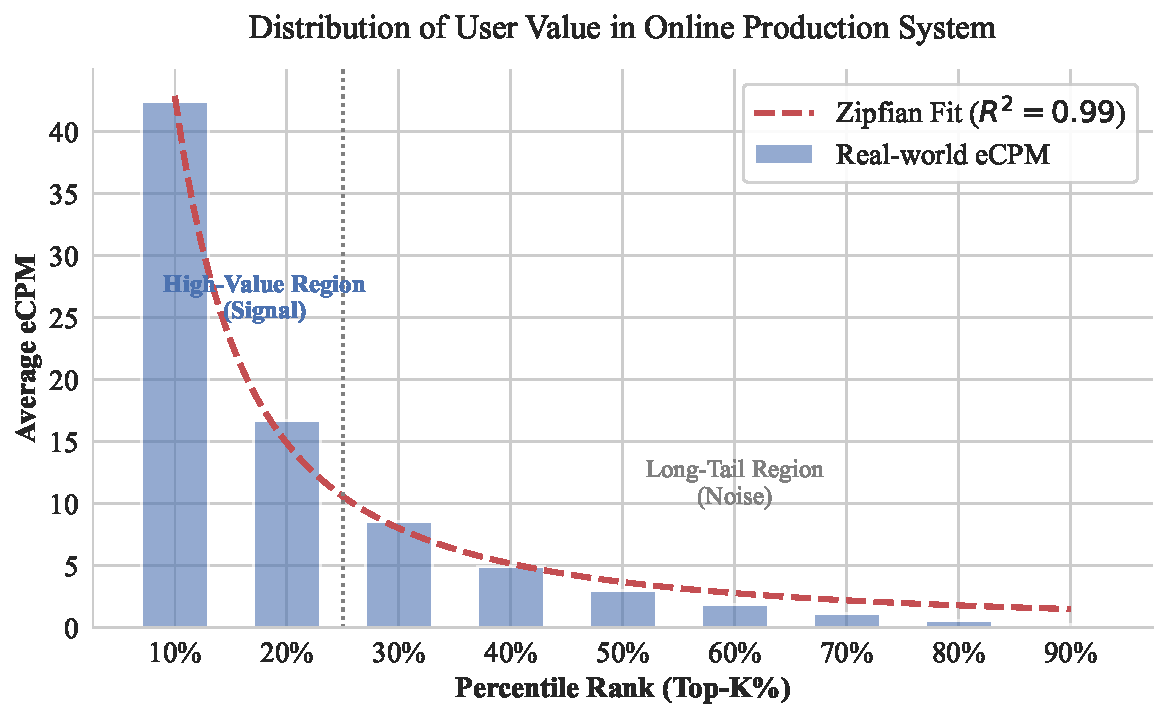
\includegraphics[width=0.9\linewidth]{figures/zipfian_distribution.pdf}
  \caption{Collected from a large-scale industrial recommendation system, the eCPM statistics exhibit a strict \textbf{Zipfian distribution}. High-value signals are extremely sparse, while the vast majority of interactions constitute low-value noise.}
  \label{fig:zipfian_intro}
\end{figure}
Our contributions are summarized as follows:

\vspace{-7pt}
\begin{itemize}\setlength{\itemsep}{0pt}\setlength{\parskip}{0pt}\setlength{\parsep}{0pt}
    \item \textbf{Theoretical Foundation:} We establish the \textit{Divergence Theory of Repulsive Optimization}, proving that negative gradients in off-policy training inevitably drive exponential intensity explosion. This theory provides a unified lens that not only explains the failure of standard methods but also identifies the ``Noise Cloning'' limit of soft-weighting strategies.

    \item \textbf{Principled Formulation:} To resolve the \textit{Convergence-Denoising Paradox}, we reformulate the learning objective as an \textbf{Optimistic Distributionally Robust Optimization (DRO)} problem. We derive that the closed-form solution is strictly a hard-filtered distribution, thereby providing the missing theoretical justification for ``hard'' denoising over ``soft'' relaxation.

    \item \textbf{Methodological Innovation:} We propose \textbf{DRPO}, a framework that operationalizes this theoretical insight via a \textbf{decoupled architecture}. By separating \textit{what to learn} (via DRO-based hard filtering) from \textit{how to learn} (via adaptive trust regions), DRPO effectively isolates high-quality behaviors while ensuring robust convergence.

    \item \textbf{Empirical Superiority:} Extensive experiments on high-fidelity industrial simulations demonstrate that DRPO achieves state-of-the-art performance. Crucially, it exhibits superior robustness in extreme noise (Zipfian) regimes where baselines collapse.
    % and generalizes effectively to broader continuous control tasks.
\end{itemize}


% ------------------------------------------------------------------
% SECTION 2: PRELIMINARIES
% ------------------------------------------------------------------

% ------------------------------------------------------------------
% SECTION 2: PRELIMINARIES
% ------------------------------------------------------------------

\section{Preliminaries}
\label{sec:preliminaries}

% ------------------------------------------------------------------
% SECTION 2: PRELIMINARIES
% ------------------------------------------------------------------

\subsection{Problem Formulation: Generative Recommendation}

We formulate generative recommendation as a continuous control problem. Let $\mathcal{S}$ be the state space encapsulating user context (e.g., behavior sequences).
Unlike discrete retrieval, we define the action space $\mathcal{A} = \mathbb{R}^d$ as a continuous embedding manifold, allowing the policy to capture dense semantic relationships~\cite{dulac2015deep}.
The generative policy $\pi_\theta(\cdot|s)$ maps a state $s$ to a latent item vector $a \in \mathcal{A}$, which is subsequently decoded into a concrete item via Maximum Inner Product Search (MIPS)~\cite{johnson2019billion}.

To align with industrial standards and facilitate the geometric analysis in Section~\ref{sec:theory}, we model the policy as a multivariate Gaussian:
\begin{equation}
\label{eq:gaussian_policy}
\begin{split}
    \pi_\theta(a|s) &= \mathcal{N}(\mu_\theta(s), \Sigma) \\
    &\propto \exp\left(-\frac{1}{2} \|a - \mu_\theta(s)\|_{\Sigma^{-1}}^2 \right),
\end{split}
\end{equation}
where $\mu_\theta(s)$ denotes the deterministic embedding generated by the network, and $\Sigma$ is the covariance matrix.
Crucially, this formulation implies that the gradient scale is inversely proportional to the variance ($\Sigma^{-1}$), a property that creates a fundamental sensitivity trade-off we analyze later.
The objective is to maximize the expected return: $J(\pi) = \mathbb{E}_{\tau \sim \pi} [\sum R(s,a)]$.

\subsection{Offline Reinforcement Learning Framework}

We adopt the offline RL setting, learning from a static dataset $\mathcal{D} = \{(s_i, a_i, R_i)\}$ collected by a behavior policy $\pi_\beta$.
In recommender systems, $\pi_\beta$ is typically a noisy mixture, resulting in a log distribution that is heavily skewed.
Standard methods optimize the policy via the Policy Gradient (PG)~\cite{sutton1999policy}:
\begin{equation}
    \nabla J(\theta) \approx \mathbb{E}_{(s,a) \sim \mathcal{D}} \left[ \hat{A}(s,a) \nabla_\theta \log \pi_\theta(a|s) \right],
    \label{eq:pg}
\end{equation}
where the advantage $\hat{A}(s,a) = R(s,a) - b(s)$ is centered via a baseline $b(s)$ (e.g., value function $V(s)$ or batch average).

\textbf{Critically, while the advantage is theoretically zero-mean, the Zipfian nature of recommendation data creates a severe \textit{Frequency Imbalance} (as shown in Figure~\ref{fig:zipfian_intro}).}
Since valid high-reward signals are extremely sparse, the baseline (reflecting the average performance) typically exceeds the reward of the vast majority of noisy samples.
This means that structurally, the dataset is dominated by suboptimal interactions with negative advantages ($\hat{A} < 0$).
Consequently, the optimization landscape is governed by these high-frequency ``repulsive'' updates. As we demonstrate in Section~\ref{sec:theory}, this negative domination, coupled with the unbounded distance in continuous space, acts as the fundamental catalyst for model divergence.

% ------------------------------------------------------------------
% SECTION 3: THEORETICAL FRAMEWORK
% ------------------------------------------------------------------
\section{Theoretical Framework: The Divergence Theory}
\label{sec:theory}

In this section, we establish the \textit{Divergence Theory of Repulsive Optimization}. We model the offline policy update as a discrete dynamical system and demonstrate that in the far-field regime—a condition where policy parameters deviate significantly from the data support—the prevalence of negative advantages inherently induces expansive dynamics. This drives the policy parameters to diverge exponentially from the data distribution.

\subsection{Discrete Dynamics of Repulsion}
\label{sec:discrete_dynamics}

To analyze the update dynamics in continuous spaces, we first establish the geometric properties of the Gaussian policy defined in Eq.~\eqref{eq:gaussian_policy}~\cite{sutton2018reinforcement}.


\begin{proposition}[Geometry of the Score Function]
\label{prop:score_function_geometry}
For the Gaussian policy $\pi_\theta(a|s)$, the gradient in the joint parameter space $\theta = [\mu, \xi]^\top$ exhibits a specific \textbf{geometric structure} determined by the variance:
\begin{equation}
\nabla_{\theta} \log \pi_\theta(a|s) = \left[ \frac{a - \mu}{\sigma^2}, \frac{(a - \mu)^2}{\sigma^2} - 1 \right]^\top.
\label{eq:joint_gradient}
\end{equation}
The Hessian matrix $\mathbf{H}(\theta)$ of the negative log-likelihood defines the local curvature of the Gaussian manifold and is \textbf{Symmetric Positive Definite (SPD)}~\cite{amari1998natural}.
\end{proposition}

This joint gradient corresponds to the \textbf{Score Function}. Proposition \ref{prop:score_function_geometry} reveals its physical meaning: the update direction is not arbitrary but is geometrically shaped by the \textbf{curvature $\mathbf{H}(\theta)$}, which dictates the coupled evolution of mean and variance.

\textit{Proof.} The derivation is straightforward from the Gaussian log-likelihood gradient. See Appendix~\ref{app:derivations} for details.

\begin{theorem}[Sign-Dependent Dynamics]
\label{thm:sign_dependent_dynamics}
Consider the discrete update rule $\theta_{t+1} \leftarrow \theta_t + \eta \hat{A} \nabla_\theta \log \pi_\theta$ for a single sample $(s,a)$. The asymptotic behavior of the system is determined solely by the sign of $\hat{A}$:
\begin{itemize}\setlength{\itemsep}{0pt}\setlength{\parskip}{0pt}\setlength{\parsep}{0pt}
\item \textbf{Case 1: Repulsive Regime ($\hat{A} < 0$)}. The transition matrix is $\mathbf{T}_{neg} = \mathbf{I} + \eta |\hat{A}| \mathbf{H}(\theta)$. Since $\mathbf{H}(\theta)$ is positive definite, $\rho(\mathbf{T}_{neg}) > 1$. The system forms an \textbf{Expansion Mapping}, causing the parameter vector $\theta_t$ to diverge. This divergence creates a positive feedback loop where the joint gradient norm $\|\nabla_{\theta} \log \pi\|$ increases with distance, leading to \textbf{Gradient Explosion}.
\item \textbf{Case 2: Attractive Regime ($\hat{A} > 0$)}. The transition matrix is $\mathbf{T}_{pos} = \mathbf{I} - \eta |\hat{A}| \mathbf{H}(\theta)$. For a valid learning rate, $\rho(\mathbf{T}_{pos}) < 1$. The system forms a \textbf{Contraction Mapping}, causing $\theta_t$ to converge. As the distance in parameter space decreases, the update signal naturally decays, resulting in \textbf{Asymptotic Gradient Attenuation}.
\end{itemize}
\end{theorem}

This theorem establishes that negative advantages inherently act as a repulsive force in the joint parameter space. We next analyze the consequences of this force in the offline setting.

\textit{Proof.} See Appendix~\ref{app:proof_dynamics}.


\subsection{Asymptotic Analysis of Gradient Flow}

The core pathology of off-policy optimization stems from the inherent dynamical asymmetry revealed in Theorem \ref{thm:sign_dependent_dynamics}. The learning process exhibits a critical temporal divergence:
\begin{itemize}\setlength{\itemsep}{0pt}\setlength{\parskip}{0pt}\setlength{\parsep}{0pt}
    \item \textbf{Attenuation of Attraction:} For high-quality samples ($\hat{A}>0$), the contraction mapping ensures that as $\theta_t$ converges to the target, the gradient $\|\nabla_\theta \log \pi\|$ decays exponentially.
    \item \textbf{Amplification of Repulsion:} Conversely, for suboptimal samples ($\hat{A}<0$), the expansion mapping drives $\theta_t$ away. Crucially, the gradient norm $\|\nabla_\theta \log \pi\|$ grows due to the increasing distance.
\end{itemize}

For a persistent negative sample, the joint displacement $\Delta_t$ grows geometrically: $\|\Delta_t\| \propto \rho^t$ (where $\rho > 1$).
Recalling the score function geometry (Eq.~\ref{eq:joint_gradient}), the gradient w.r.t. $\mu$ scales linearly with displacement, whereas the gradient w.r.t. the log-variance $\xi$ is driven by the \textbf{squared term} $(a-\mu)^2$, thus scaling \textbf{quadratically} ($\nabla_\xi \propto \|\Delta\|^2$).
This mechanism explains why the gradient norm explodes much faster than the parameter displacement itself.

\begin{corollary}[Quadratic Gradient Explosion]
\label{cor:intensity_explosion}
Let $\Delta_t$ be the displacement under repulsive dynamics. Dominated by the quadratic curvature of the variance parameter, the joint gradient norm exhibits \textbf{quadratic exponential growth}:
\begin{equation}
    \|\nabla_{\theta} \log \pi_t\| \propto \frac{\|\Delta_0\|^2}{\sigma^2} \cdot \rho^{2t}.
\end{equation}
Since $\rho > 1$, the gradient magnitude diverges at a rate of $\mathcal{O}(\rho^{2t})$, analytically guaranteeing numerical overflow regardless of bounded variance expansion.
\end{corollary}

\begin{theorem}[Contraction-Induced Fragility]
\label{thm:contraction_fragility}
Consider the convergence of the policy on positive samples such that $\sigma_t \to 0$. The sensitivity of the policy to any fixed negative sample $a_{neg}$ (where $\|a_{neg} - \mu\| > \epsilon$) becomes unbounded. Specifically, the gradient magnitude acts as a barrier function with respect to variance:
\begin{equation}
    \lim_{\sigma \to 0} \|\nabla_{\theta} \log \pi(a_{neg})\| = \infty.
\end{equation}
Consequently, higher confidence on in-distribution data (lower $\sigma$) mathematically necessitates unbounded fragility to out-of-distribution repulsive noise, establishing the structural paradox of standard off-policy learning.
\end{theorem}
\textit{Proof.} See Appendix~\ref{app:proof_fragility}.

\begin{corollary}[Asymptotic Signal-to-Noise Collapse]
\label{cor:repulsive_dominance}
Combining the asymptotic gradient attenuation on positive samples ($\|\nabla_{\theta} \log \pi(a_{pos})\| \to 0$) with the hypersensitivity derived in Theorem~\ref{thm:contraction_fragility}, the \textbf{Repulsion-to-Attraction Ratio} diverges:
\begin{equation}
\lim_{t \to \infty} \frac{\|\nabla_\theta \log \pi_t(a_{neg})\|}{\|\nabla_\theta \log \pi_t(a_{pos})\|} = \infty.
\end{equation}
This confirms that the optimization landscape inevitably becomes dominated by repulsive noise, drowning out the expert signal.
\end{corollary}

\subsection{Why On-Policy Optimization Converges}
\label{sec:on_policy_contrast}

Standard on-policy gradient methods (e.g., PPO~\cite{schulman2017proximal}) also utilize negative advantages but typically maintain stability. This is due to the \textbf{stationarity of the sampling distribution} relative to the policy.

\begin{proposition}[Translation Invariance of On-Policy Gradients]
\label{prop:on_policy_stationarity}
Unlike the expansive dynamics in off-policy regimes, on-policy optimization satisfies \textbf{Gradient Translation Invariance}.
Since the action $a$ is sampled from $\pi_{\theta_t}$ itself, the expected gradient norm depends \textbf{solely} on the covariance $\Sigma_t$, and is \textbf{independent} of the parameter's absolute position $\mu_t$:
\begin{equation}
    \mathbb{E}_{a \sim \pi_{\theta_t}} \left[ \|\nabla_\mu \log \pi_{\theta_t}(a)\|^2 \right] = \text{tr}(\Sigma_t^{-1}).
\end{equation}
This strictly bounded expectation prevents the accumulation of expansive error, guaranteeing numerical stability regardless of where the policy moves in the embedding space.
\end{proposition}


\subsection{The Convergence-Denoising Paradox: Limitations of Soft De-Repulsion}

Existing methods (e.g., AWR~\cite{peng2019advantage}, AsymRe~\cite{asymre}) rely on soft weights $w \in (0, 1]$ to mitigate divergence. We rigorously analyze their limitation by decomposing the gradient into a \textbf{Signal Force} ($\mathbf{g}_{\text{sig}}$) from sparse high-quality data $\mathcal{D}^+$ and a \textbf{Residual Noise Force} ($\mathbf{g}_{\text{noise}}$) from dominant suboptimal data $\mathcal{D}^-$:
\begin{equation}
\label{eq:grad_decomp}
\begin{aligned}
    \nabla J \approx \underbrace{\sum_{x \in \mathcal{D}^+} w_i \nabla \log \pi}_{\mathbf{g}_{\text{sig}}} + \underbrace{\sum_{x \in \mathcal{D}^-} w_j \nabla \log \pi}_{\mathbf{g}_{\text{noise}}}.
\end{aligned}
\end{equation}
This decomposition reveals the paradox driven by the \textbf{Zipfian Volume Effect} ($|\mathcal{D}^-| \gg |\mathcal{D}^+|$).
\textbf{1) Noise Cloning:} Despite individual attenuation ($w_j \to \epsilon$), the \textit{aggregate} accumulation over the massive $\mathcal{D}^-$ ensures that $\|\mathbf{g}_{\text{noise}}\|$ remains significant, biasing the equilibrium towards noise.
\textbf{2) Variance Collapse:} To strictly eliminate $\mathbf{g}_{\text{noise}}$, one must enforce mathematically sharp weights ($w_j \to 0$). However, this reduces the effective sample size, triggering the variance explosion predicted by \textbf{Theorem~\ref{thm:contraction_fragility}}.
Standard methods are thus trapped between \textit{biased convergence} and \textit{high-variance collapse}. This necessitates the distributional hard-filtering approach proposed in our DRPO framework.

% ------------------------------------------------------------------
% SECTION 4: METHODOLOGY
% ------------------------------------------------------------------

\section{Methodology: Distributionally Robust Policy Optimization}
\label{sec:methodology}

Motivated by the theoretical analysis in Section~\ref{sec:theory}, we propose Distributionally Robust Policy Optimization (DRPO). To resolve the Convergence-Denoising Paradox, DRPO abandons the monolithic soft-weighting paradigm in favor of a \textit{decoupled architecture}. We first formulate an Optimistic DRO objective to rigorously derive a hard-filtering strategy for noise rejection (Section~\ref{sec:dro_formulation}). On top of this filtered distribution, we then construct an adaptive trust-region optimizer to ensure stable convergence within the identified signal manifold (Section~\ref{sec:dynamic_curriculum}).



\subsection{The Denoising Objective: Optimistic DRO}
\label{sec:dro_formulation}

Beyond the inherent divergence analyzed in Section~\ref{sec:theory}, the fundamental limitation of Soft De-Repulsion strategies (e.g., AWR, AsymRE) lies in the learning objective itself. These MLE-based paradigms inherently aim to fit the observable behavior distribution $P_{\text{data}}$. However, in generative recommendation, $P_{\text{data}}$ is merely a noisy proxy entangling the optimal strategy with suboptimal behaviors. Therefore, we propose a paradigm shift from ``fitting the noisy proxy'' to ``recovering the latent ideal.''

To operationalize this, we posit a latent ``ideal distribution'' $Q$ hidden within the noisy behavior data. Instead of indiscriminately minimizing divergence from the entire $P_{\text{data}}$, we formulate the target identification as an \textbf{Optimistic Distributionally Robust Optimization (DRO)} problem\cite{rahimian2019distributionally}. We seek the distribution $Q$ that maximizes expected return, subject to being a valid sub-distribution of the behavior policy:
\begin{equation}
\label{eq:optimistic_dro}
    \max_{Q} \; \mathbb{E}_{(s,a) \sim Q} [R(s,a)], \quad \text{s.t.} \quad Q \in \mathcal{U}_\kappa(P_{\text{data}}),
\end{equation}
where the uncertainty set is constrained by the \textbf{Probability Density Ratio}:
\begin{equation}
    \mathcal{U}_\kappa(P_{\text{data}}) \triangleq \left\{Q : \frac{dQ(s,a)}{dP_{\text{data}}(s,a)} \le \frac{1}{\kappa}, \quad \int dQ=1 \right\}.
\end{equation}
Here, $\kappa \in (0, 1]$ represents the trust-region hyperparameter. The constraint enforces \textbf{Bounded Importance Weights}, ensuring that the learned distribution $Q$ cannot arbitrarily hallucinate mass in regions unsupported by data, but can amplify the density of high-quality regions by a factor of up to $1/\kappa$.

\textbf{Optimistic vs. Pessimistic:} Unlike conventional DRO which adopts a \textit{max-min} (pessimistic) objective to defend against worst-case perturbations, our formulation is \textit{optimistic} (max-max), explicitly seeking the ``best-case'' sub-distribution to filter out the heavy-tailed noise.

\begin{theorem}[Optimality of Hard Filtering]
\label{thm:hard_filtering_solution}
As proven in \textbf{Appendix~\ref{app:proof_theorem_4_1}}, the closed-form solution $Q^*$ to this objective is strictly a \textbf{Hard-Thresholding Distribution}:
\begin{equation}
    Q^*(s,a) \propto P_{\text{data}}(s,a) \cdot \mathbb{I}\left( R(s,a) \ge R_{1-\kappa} \right),
\end{equation}
where $R_{1-\kappa}$ is the $(1-\kappa)$-quantile of the reward distribution. This theoretically establishes ``Hard Filtering'' (Top-$\kappa$ truncation) as the exact mathematical solution to the Optimistic DRO problem.
\end{theorem}


\subsection{Variational Top-$\kappa$ Optimization via CVaR}
\label{sec:cvar_dual}

While Theorem \ref{thm:hard_filtering_solution} establishes the theoretical optimality of Hard Filtering, implementing it efficiently requires a tractable formulation. We leverage the \textbf{Variational Dual Form} of Optimistic CVaR~\cite{rockafellar2000optimization} (derived in \textbf{Appendix~\ref{app:proof_proposition_4_2}}) to construct a robust two-step optimization process.

First, we identify the signal manifold by solving the variational dual problem on the batch data. This effectively acts as an \textbf{Adaptive Quality Baseline}, where the auxiliary variable $\nu$ converges to the $(1-\kappa)$-quantile (Value-at-Risk):
\begin{equation}
\label{eq:dual_threshold}
\begin{split}
    \nu^* &= \arg\min_{\nu} \big\{ \nu + \kappa^{-1} \mathbb{E}_{\mathcal{D}} [ (R - \nu)_+ ] \big\} \\
          &\implies \nu^* = \text{Top-}\kappa \text{ Threshold}.
\end{split}
\end{equation}

With the optimal threshold $\nu^*$ determined, we project the policy onto the identified signal manifold. The learning objective becomes a \textbf{Truncated Weighted Regression}, maximizing the log-likelihood of high-reward transitions:
\begin{equation}
\label{eq:variational_objective}
    J(\theta) = \kappa^{-1} \mathbb{E}_{(s,a) \sim \mathcal{D}} \Big[ (R(s,a) - \nu^*)_+ \cdot \log \pi_\theta(a|s) \Big].
\end{equation}

The resulting gradient update rule fundamentally resolves the ``Repulsive Force'' paradox:
\begin{equation}
\label{eq:drpo_gradient}
    \nabla_\theta J \approx \kappa^{-1} \sum_{i \in \mathcal{B} : R_i \ge \nu^*} (R_i - \nu^*) \nabla_\theta \log \pi_\theta(a_i|s_i).
\end{equation}

\begin{itemize}
    \item \textbf{Elimination of Repulsion:} By strictly filtering out samples where $R_i < \nu^*$, we ensure the effective advantage term $(R_i - \nu^*)$ is always \textbf{non-negative}. This physically prevents the variance parameter from receiving expansive gradients, stabilizing the learning dynamics.
    \item \textbf{Prevention of Noise Cloning:} The threshold $\nu^*$ acts as a hard gatekeeper. Unlike soft-weighting methods, our formulation strictly zeroes out gradients from the noise distribution, ensuring the policy learns exclusively from the \textbf{Signal Manifold}.
\end{itemize}

\textbf{Remark (Theoretical Connection).} This derivation offers a rigorous grounding for heuristic methods like \textbf{AsymRe} ~\cite{asymre}. AsymRe can be mathematically interpreted as a ``Soft Relaxation'' of our Optimistic DRO solution. While empirically effective in mild noise, its lack of a strict truncation mechanism (hard sparsity) means it cannot theoretically guarantee the elimination of repulsive forces in heavy-tailed noise regimes.

\subsection{Variance-Guided Dynamic Curriculum and Generalization}
\label{sec:dynamic_curriculum}

\paragraph{Adaptive Curriculum.}
Solving the variational dual requires determining the optimal threshold $\nu^*$, which corresponds to the $(1-\kappa)$-quantile of the batch rewards. However, a static $\kappa$ is suboptimal as the signal-to-noise ratio fluctuates during training. To ensure consistent gradient fidelity, we propose a simple yet effective \textbf{Variance-Guided} mechanism:
\begin{equation}
    \kappa_t \propto \text{Var}(R_t).
\end{equation}
This rule dynamically scales the effective sample size ($N \cdot \kappa$) against noise. In high-variance stages, the algorithm expands $\kappa$ to stabilize estimation (Bias-Variance trade-off); as the policy converges and variance drops, $\kappa$ naturally shrinks to exploit peak performance. This induces an automated \textbf{``Easy-to-Hard'' curriculum}~\cite{bengio2009curriculum}, balancing stability and optimality without complex hyperparameter tuning.

\paragraph{Generalized Paradigm.}
The core insight of ``Dynamic Hard Filtering'' establishes a generalizable paradigm for off-policy learning. By abstracting the update rule, we derive variants adaptable to different inductive biases:
\vspace{-5pt}
\begin{itemize}\setlength{\itemsep}{0pt}\setlength{\parskip}{0pt}\setlength{\parsep}{0pt}
    \item \textbf{DRPO-Exp (Hard-Cut, Soft-Focus):} While our primary derivation yields a linear weighting scheme $(R-\nu^*)_+$, one can apply exponential weighting $w_i \propto \exp(R_i/\tau)$ \textit{strictly within} the filtered Top-$\kappa$ manifold. As rigorously justified in \textbf{Appendix~\ref{app:proof_drpo_exp}}, this variant introduces an additional \textbf{KL-regularization term}~\cite{peters2010relative} inside the signal manifold. This sharpens the focus on the absolute best samples, proving particularly beneficial for heavy-tailed distributions where the Top-$\kappa$ set itself retains high variance.
    \item \textbf{DRPO-Q (Long-Term Value):} To extend DRPO to multi-step Reinforcement Learning tasks where trajectory returns are unavailable, the immediate reward $R$ can be substituted with a learned Q-value $Q_\phi(s,a)$ (e.g., via IQL~\cite{kostrikov2021offline} backbones). This variant captures long-term dependencies while maintaining the robustness benefits of hard filtering, effectively bridging the gap between generative recommendation and general offline RL.
\end{itemize}

\subsection{Algorithm Summary}
\label{sec:algorithm_summary}

The complete DRPO algorithm integrates the Variational Top-$\kappa$ Optimization (Section \ref{sec:cvar_dual}) with the Variance-Guided Curriculum (Section \ref{sec:dynamic_curriculum}). The full procedure is detailed in \textbf{Algorithm~\ref{alg:drpo}} (Appendix \ref{app:algorithm_details}). The method is computationally efficient, with negligible overhead from batch-wise sorting ($O(N \log N)$), and maintains minimal complexity, facilitating seamless integration into various generative recommendation backbones.


\section{Experiments}
\label{sec:experiments}

In this section, we present extensive experiments to validate the theoretical claims and the effectiveness of DRPO. We first verify the Divergence Theory by visualizing the phantom gradients (RQ1). We then evaluate the robustness of DRPO against noise injection (RQ2), followed by a comparison with state-of-the-art methods on standard benchmarks (RQ3). Finally, we demonstrate the superiority of DRPO in offline-to-online evolutionary dynamics (RQ4).

\subsection{Experimental Setup}
\label{sec:exp_setup}

\textbf{High-Fidelity Simulation (RecSim).}
Standard public datasets are static and fail to capture the stochastic feedback loops inherent in industrial systems. To bridge this gap, we utilize \textbf{RecSim} (detailed in \textbf{Appendix~\ref{app:simulation}}), a high-fidelity simulator designed to replicate the topology and noise profiles of production environments.\footnote{To facilitate reproducibility and support future research on robust RL, the source code and environment configurations will be made publicly available.} RecSim operates in a continuous embedding space ($d=128$) and employs a mixed-strategy logging agent to generate \textbf{Zipfian-distributed} data. This setup strictly enforces the ``data curse,'' where high-value signals are sparse and the distribution is dominated by suboptimal noise.

\textbf{Data Scenarios.}
We evaluate algorithms across two distinct regimes mirroring real-world industrial stages:
(1) \textbf{Medium Quality (Impression Logs):} Simulates post-exposure feedback where data is biased but contains valid signals (mixed strategy); and
(2) \textbf{Extreme Noisy (Full Corpus Retrieval):} Simulates the initial retrieval stage dominated by random exploration ($90\%$ noise ratio), serving as a critical stress test for robustness.

\textbf{Baselines.}
We compare DRPO against a comprehensive suite of 8 representative algorithms spanning three paradigms:
(1) \textbf{Standard Off-Policy RL:} \textbf{Advantage Policy Gradient(APG)};
(2) \textbf{Regularized Imitation:} \textbf{BC}, \textbf{CRR}~\cite{wang2020critic}, and \textbf{BPPO}~\cite{zhuang2023behavior};
and (3) \textbf{Soft-Weighting \& Value-Based Methods:} \textbf{AWR}~\cite{peng2019advantage}, \textbf{IQL}~\cite{kostrikov2021offline}, \textbf{AsymRe}, and \textbf{Adaptive BC}.
Implementation details and hyperparameter settings are provided in \textbf{Appendix~\ref{app:algorithm_details}}.

We implement all algorithms using PyTorch on a single NVIDIA GPU. For fair comparison, all methods share the same backbone network architecture (a 2-layer MLP with 128 hidden units). The specific hyperparameter configurations for our proposed DRPO, its variant DRPO-exp, and other baselines are detailed in \textbf{Appendix~\ref{app:hyperparams}}.


\subsection{RQ1: Empirical Verification of Divergence Theory}
\label{sec:phantom_gradient}

To empirically validate the \textit{Divergence Theory}, we analyze the optimization dynamics using a \textbf{``Phantom Gradient''} monitor: the policy is trained exclusively on positive samples, while we concurrently track the gradients of negative samples without applying them.
\begin{figure}[t]
  \centering
  % --- 左图 (a) ---
  \begin{subfigure}[b]{0.49\linewidth}
    \centering
    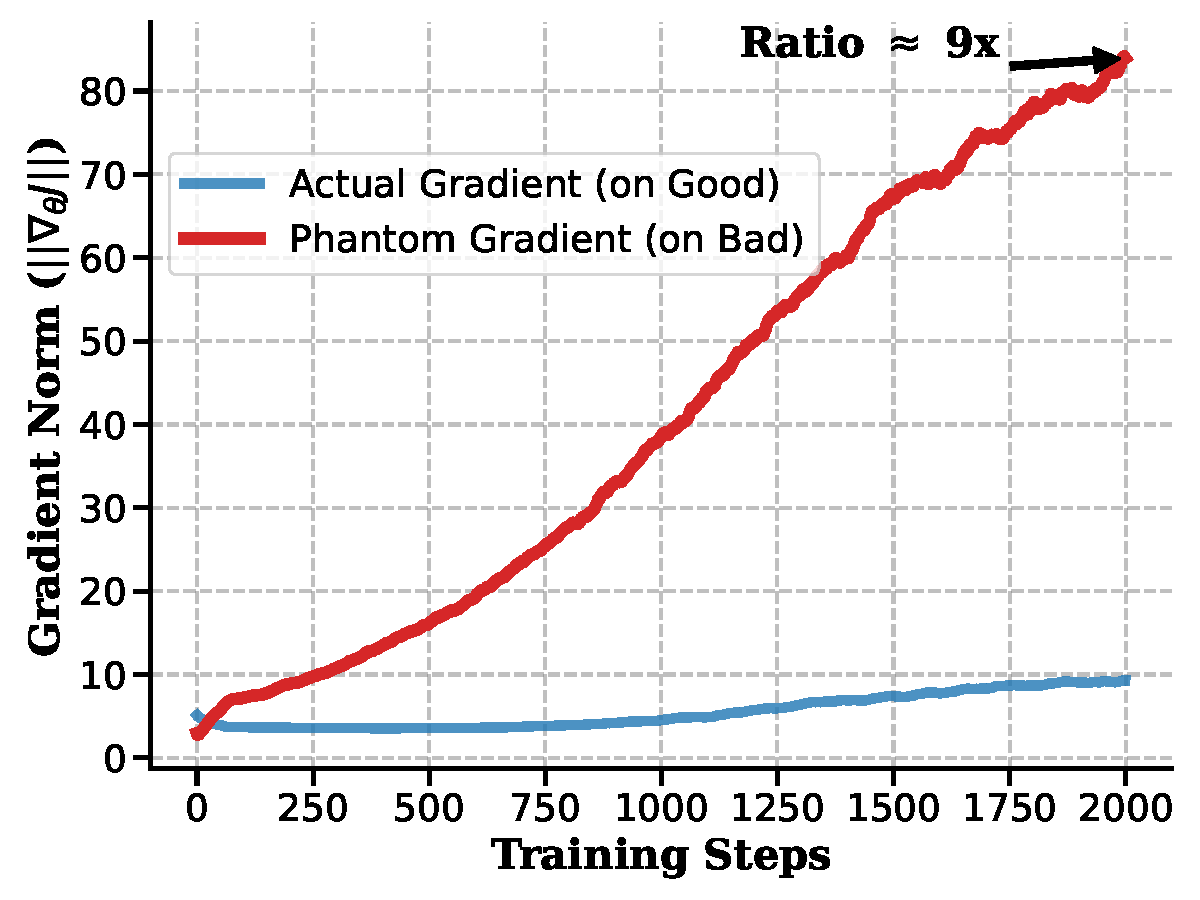
\includegraphics[width=\linewidth]{figures/2_gradient_paper.pdf}
    \caption{Gradient Explosion} % 从平淡的 Norm 改为更有力的 Explosion
    \label{fig:phantom_gradient}
  \end{subfigure}
  \hfill % 左右撑开
  % --- 右图 (b) ---
  \begin{subfigure}[b]{0.49\linewidth}
    \centering
    
\includegraphics[width=\linewidth]{figures/3_force_paper.pdf}
    \caption{Structural Collapse} % 对应 Sigma 的坍塌和 Mu 的逃逸，非常精准
    \label{fig:force_analysis}
  \end{subfigure}

  \vspace{-0.2cm}

  % --- 主 Caption ---
  \caption{\textbf{Verification of Divergence Theory.}
  (a) \textbf{Gradient Explosion:} Negative gradients explode ($\approx 9\times$).
(b) \textbf{Structural Expansion:} Both $\mu$ and $\sigma$ expand. Crucially, the repulsive imbalance on $\sigma$ (Ratio $\approx 58\times$) is far more severe than on $\mu$ (Ratio $\approx 2\times$).}  \label{fig:divergence_verification}
\end{figure}
\textbf{The Force (Gradient Explosion).}
As shown in Figure~\ref{fig:divergence_verification}(a), while gradients from positive samples converge stably, the phantom repulsive gradients exhibit \textbf{exponential growth}. This confirms Theorem~\ref{thm:sign_dependent_dynamics}: the further the policy moves from a negative sample, the stronger the repulsive force becomes, creating a self-reinforcing expansion loop that inevitably leads to divergence if not rigorously filtered.

\textbf{The State (Structural Collapse).}
We further decompose this divergence into structural components (Figure~\ref{fig:divergence_verification}(b)).
First, the repulsive force on $\mu$ scales quadratically with displacement, driving the embedding norm toward overflow (\textbf{Corollary~\ref{cor:intensity_explosion}}).
Crucially, the gradients w.r.t. $\sigma$ explode even more aggressively, with a repulsive-to-attractive ratio exceeding $\mathbf{58\times}$.
This strictly corroborates \textbf{Theorem~\ref{thm:contraction_fragility}}: as the policy becomes confident on in-distribution data ($\sigma \to 0$), it mathematically necessitates unbounded hypersensitivity to out-of-distribution noise.
This structural pathology explains why soft-weighting methods fail—any non-zero weight assigned to noise eventually faces an infinite variance multiplier ($\sigma^{-2}$), which only discrete hard filtering can physically sever.



% \subsubsection{Oracle Validation}
% To rigorously assess the denoising capability of DRPO, we introduce an \textbf{"Oracle" baseline}, where the model is trained only on manually filtered high-quality data (Gold Standard). We compare this against DRPO (trained on mixed noisy data) and AWR (trained on mixed noisy data).
% Our results show that the learning curve of DRPO closely tracks the Oracle baseline, significantly outperforming AWR. This indicates that DRPO's hard filtering mechanism is mathematically equivalent to "perfect" manual noise removal, effectively recovering the latent optimal distribution $Q^*$ from the noisy mixture $P_{\text{data}}$.

\subsection{RQ2: Main Performance Comparison}
\label{sec:main_results}

Table~\ref{tab:main_results} compares DRPO against baselines across two distinct regimes.

\textbf{Empirical Verification of Divergence.}
Standard \textbf{APG} suffers catastrophic failure across both scenarios (Reward $\approx 0.01$), with massive semantic deviation (Dist. $>3.8$). This provides direct empirical validation of our Divergence Theory: without explicit constraints, repulsive gradients inherently drive parameters toward numerical overflow, rendering naive off-policy learning futile.

\textbf{Robustness in Extreme Noise.}
The distinction between methods becomes stark in the \textbf{Extreme Noisy} setting.
While regularized methods (e.g., IQL, Adaptive BC) perform adequately in medium quality, they degrade significantly under heavy noise. Soft-weighting strategies (AWR, AsymRe) fail to suppress the overwhelming noise, exhibiting distinct ``Noise Cloning'' symptoms.
In sharp contrast, \textbf{DRPO-Exp} maintains SOTA performance (Reward \textbf{0.379}), indistinguishable from the medium-quality setting. This confirms that \textbf{Hard Filtering} is not merely an optimization trick but a mathematically necessary condition for survival in heavy-tailed noise environments, effectively recovering the sparse signal where soft relaxations fail.Notably, Adaptive BC achieves runner-up performance solely via supervised learning, directly validating the standalone efficacy of our hard filtering mechanism

% 确保导言区有这些包
% \usepackage{colortbl}
% \usepackage{xcolor}

% 务必在导言区添加: \usepackage{booktabs}

\begin{table*}[t]
\centering
\caption{\textbf{Comprehensive Performance Comparison.}
We evaluate algorithms in \textbf{Medium Quality} and \textbf{Extreme Noisy} scenarios.
\textbf{DRPO} and \textbf{DRPO-Exp} consistently achieve the top-2 performance.
(Best results are \textbf{bolded}, second-best are \underline{underlined}).
Notably, \textbf{Adapt. BC} outperforms complex RL baselines, validating the efficacy of our filtering mechanism.}
\label{tab:main_results}
\resizebox{\textwidth}{!}{
\begin{tabular}{llcccccccc} % 去掉竖线，调整列数
\toprule
\multirow{2}{*}{Scenario} & \multirow{2}{*}{Metrics} & \multicolumn{6}{c}{Baselines} & \multicolumn{2}{c}{Ours} \\
\cmidrule(lr){3-8} \cmidrule(lr){9-10} % 分组横线
 & & BC & CRR & BPPO & AWR & IQL & Adapt. BC & \textbf{DRPO-Exp} & \textbf{DRPO} \\
\midrule
\multirow{2}{*}{\shortstack[l]{\textbf{Medium Quality}\\(Mixed Strategy)}}
& Reward $\uparrow$ & $0.338$ & $0.222$ & $0.341$ & $0.333$ & $0.337$ & $0.367$ & \underline{$0.372$} & \textbf{0.374} \\
& eCPM $\uparrow$   & $1.69$  & $1.11$  & $1.70$  & $1.66$  & $1.68$  & $1.84$  & \underline{$1.86$}  & \textbf{1.87} \\
\midrule
\multirow{2}{*}{\shortstack[l]{\textbf{Extreme Noisy}\\(Noise Dominated)}}
& Reward $\uparrow$ & $0.268$ & $0.217$ & $0.124$ & $0.254$ & $0.289$ & $0.297$ & \textbf{0.318} & \underline{$0.308$} \\
& eCPM $\uparrow$   & $1.34$  & $1.08$  & $0.62$  & $1.27$  & $1.44$  & $1.48$  & \textbf{1.59}  & \underline{$1.54$} \\
\bottomrule
\end{tabular}
}
\vspace{-10pt} % 如果还觉得占地，可以调整这个负值，比如 -15pt
\end{table*}
\subsection{RQ3: Robustness and Mechanism Analysis}

\subsubsection{Noise Injection Study}
\begin{figure}[htbp]
  \centering
  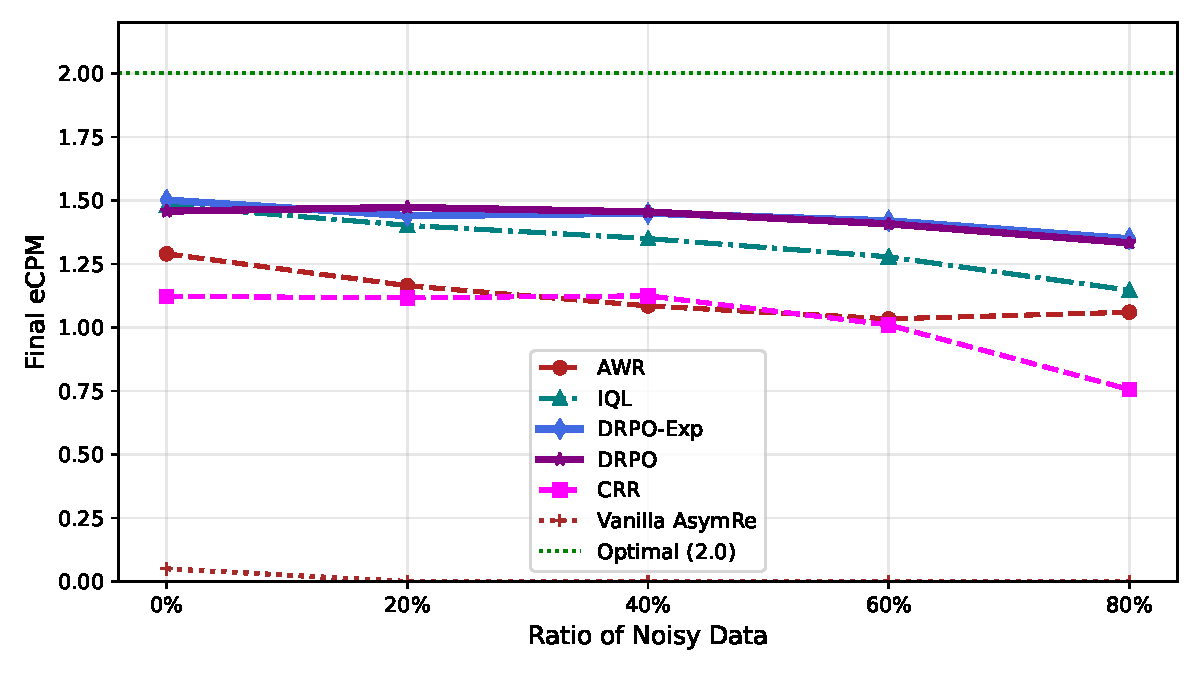
\includegraphics[width=0.9\linewidth]{figures/recsys_extended_benchmark.pdf}
  \caption{Robustness against Noise Injection. DRPO maintains performance as noise increases, whereas soft-weighting methods degrade significantly.}
  \vspace{-10pt}
  \label{fig:noise_robustness}
\end{figure}
To evaluate robustness, we artificially inject varying ratios of low-quality data (Noise Ratio from 0\% to 80%) into the training set. Figure~\ref{fig:noise_robustness} illustrates the performance drop as noise increases.
Soft-weighting methods like AWR and AsymRe suffer significant degradation, confirming our hypothesis of "Trash Cloning"—they fail to fully suppress the influence of abundant noise. Conversely, DRPO maintains consistent high performance even at 80\% noise ratio, demonstrating that the DRO-derived Hard Filtering is the robust solution for heavy-tail noise distributions.


\subsection{RQ3: Robustness and Mechanism Analysis}
\label{sec:ablation}

\textbf{Noise Tolerance (Figure~\ref{fig:noise_robustness}).}
We stress-test the algorithms by injecting varying ratios of random noise (0\% to 80\%).
Soft-weighting methods (AWR, AsymRe) degrade linearly with noise, confirming the ``Trash Cloning'' hypothesis—they fail to fully suppress the influence of abundant suboptimal data.
Conversely, \textbf{DRPO} exhibits exceptional resilience, maintaining near-optimal performance even at 80\% noise ratio. This empirically proves that the DRO-derived Hard Filtering effectively severs the tail dependency, rendering the method invariant to the volume of background noise.

\textbf{Ablation Study (Table~\ref{tab:ablation_component}).}
Consistent with the divergence risks predicted by \textbf{Theorem~\ref{thm:sign_dependent_dynamics}}, the Soft-Base is essential for preventing the collapse observed in naive hard filtering (Row 1 vs. 2).
However, stability alone is insufficient; explicitly removing the ``toxic tail'' via Hard Filtering provides a clear boost ($1.15 \to 1.31$).
Finally, our Variance-Guided Adaptive mechanism maximizes this gain (reaching \textbf{1.42}) by dynamically optimizing the signal-to-noise ratio.

To further understand the necessity of adaptivity, we analyzed fixed filtering ratios under varying noise levels (see \textbf{Appendix~\ref{app:sensitivity}}). We found that while aggressive filtering is essential for low-quality data, conservative strategies are required in high-noise regimes to prevent \textit{overfitting to stochastic reward noise}, confirming that no single fixed ratio is universally optimal.
% Further analysis in \textbf{Appendix~\ref{tab:sensitivity_sweep}} reveals that fixed ratios fail to generalize: aggressive filtering is essential to combat \textbf{poor quality data (high policy noise)}, while conservative strategies are required to prevent \textbf{overfitting to stochastic reward noise}.

\begin{table}[h]
\centering
\caption{\textbf{Ablation Study: Step-by-Step Mechanism Analysis.}
Hard Filtering alone leads to policy collapse (Row 1), while Soft-Base stabilizes training but plateaus early (Row 2).
Crucially, combining them unlocks significant gains ($1.15 \to 1.31$), with the \textbf{Adaptive mechanism} achieving peak performance by dynamically optimizing the signal-to-noise ratio.}
\vspace{-5pt}
\label{tab:ablation_component}
\begin{small}
\begin{sc}
\resizebox{\columnwidth}{!}{
\begin{tabular}{cccccc}
\toprule
\multicolumn{3}{c}{Component Configuration} & \multicolumn{2}{c}{Performance} \\
\cmidrule(r){1-3} \cmidrule(l){4-5}
Soft-Base & Hard Filter & Adaptive & True eCPM & Gap \\
\midrule
$\times$ & $\checkmark$ (Fixed) & $\times$ & $0.12$ & $-91.5\%$ \\
$\checkmark$ & $\times$ & $\times$ & $1.15$ & $-19.0\%$ \\
$\checkmark$ & $\checkmark$ (Fixed) & $\times$ & $1.31$ & $-7.7\%$ \\
\rowcolor{grayhighlight}
$\checkmark$ & $\checkmark$ (Ours) & $\checkmark$ & \textbf{1.42} & \textbf{--} \\
\bottomrule
\end{tabular}
}
\vspace{-10pt} % 如果还觉得占地，可以调整这个负值，比如 -15pt

\end{sc}
\end{small}
\end{table}

\subsection{RQ4: Offline-to-Online Evolutionary Dynamics}
\label{sec:o2o_exp}

We investigate the policy's evolution under a hybrid data stream, transitioning from static offline initialization to dynamic online interaction (Figure\ref{fig:o2o_dynamics} and Table\ref{tab:o2o_performance}).



\textbf{Mechanism: Safe Transition.}
DRPO exhibits a unique \textbf{``Self-Paced Curriculum.''}
As shown in Figure~\ref{fig:o2o_dynamics}, the \textit{Online Data Ratio} (green line)---defined as the proportion of real-time samples admitted by the hard filter---starts near zero. This indicates that our Variance-Guided mechanism detects the initial high-variance feedback and automatically tightens the trust region (low $\kappa$). This effectively acts as a ``safety gate,'' shielding the policy from collapse caused by low-quality exploration.
As the policy improves, the filter progressively admits more online samples, enabling a seamless transition that eliminates the performance dip often observed in standard fine-tuning.

\textbf{Performance: Speed and Quality.}
DRPO adapts significantly faster than baselines, demonstrating superior sample efficiency.
In the converged state (Table~\ref{tab:o2o_performance}), both \textbf{DRPO} ($1.96$) and \textbf{DRPO-Exp} ($1.93$) substantially outperform strong baselines like IQL ($1.84$) and AWR ($1.21$).
This confirms that while soft-weighting suffices for mild shifts, the heavy-tailed noise in industrial online feedback requires DRPO's hard filtration to robustly recover sparse high-value signals.

\begin{figure}[t]
    \centering
    % 左侧：图 (垂直居中)
    \begin{minipage}[c]{0.63\linewidth}
        \centering
        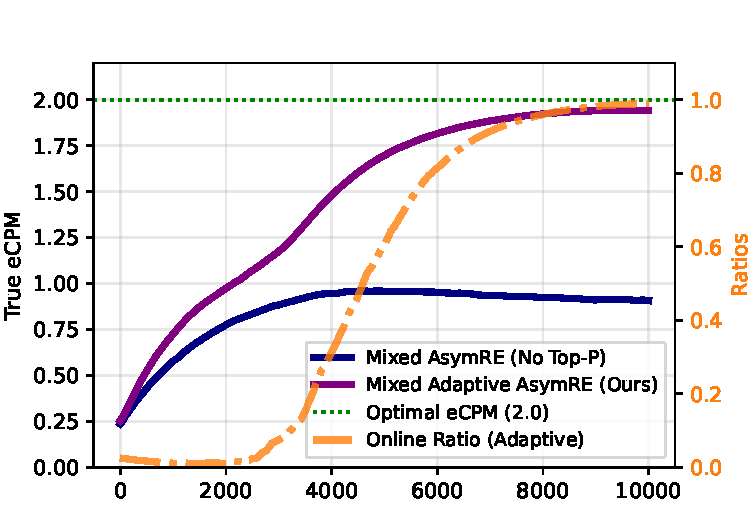
\includegraphics[width=\linewidth]{figures/recsys_ablation_analysis.pdf}
        \captionof{figure}{Evolutionary Dynamics. DRPO seamlessly transitions from offline safeguarding to online exploration.}
        \label{fig:o2o_dynamics}
    \end{minipage}
    \hfill
    % 右侧：表 (垂直居中)
    \begin{minipage}[c]{0.359\linewidth}
        \centering
        % 样式设置
        \scriptsize
        \setlength{\tabcolsep}{4pt}
        \renewcommand{\arraystretch}{0.98}

        \begin{tabular}{lc}
            % 【修改点1】指定 Toprule 宽度为 0.7pt (默认约0.8pt)
            \toprule[0.7pt]
            \textbf{Method} & \textbf{eCPM} \\

            % 【修改点2】Midrule 保持默认或稍微变细 (0.4pt)
            \midrule[0.4pt]
            AsymRe   & $1.05$ \\
            AWR      & $1.21$ \\
            IQL      & $1.84$ \\
            \midrule[0.4pt]
            \rowcolor{grayhighlight}
            \textbf{DRPO-Exp} & $1.93$ \\
            \rowcolor{grayhighlight}
            \textbf{DRPO} & \bm{$1.96$} \\

            % 【修改点3】指定 Bottomrule 宽度为 0.7pt
            \bottomrule[0.7pt]
        \end{tabular}

        \vspace{2pt}
        \captionof{table}{Converged Performance. DRPO variants consistently outperform baselines}
        \label{tab:o2o_performance}
    \end{minipage}
    \vspace{-10pt}
\end{figure}

% \subsection{Generalization on D4RL Benchmarks}

% To further demonstrate the universality and robustness of DRPO, we extend our evaluation to standard continuous control benchmarks using the D4RL suite~\cite{fu2020d4rl}. Although our primary focus is generative recommendation, the core challenge—learning from noisy, suboptimal offline data—is shared across domains. By testing on MuJoCo locomotion tasks~\cite{todorov2012mujoco}, we verify that the effectiveness of our Hard Filtering mechanism and Variance-Guided Curriculum generalizes beyond the specific structure of recommendation embeddings to general continuous action spaces.

% \begin{table}[ht]
% \caption{Normalized scores on D4RL benchmarks. We compare DRPO with standard baselines on various MuJoCo tasks. DRPO demonstrates competitive or superior performance across different environments and dataset qualities, highlighting its generalization capability.}
% \label{tab:d4rl_results}
% \begin{center}
% \begin{small}
% \begin{sc}
% \resizebox{\columnwidth}{!}{
% \begin{tabular}{lcccccc}
% \toprule
% Environment & BC & APG & AWR & IQL & AsymRe & DRPO \\
% \midrule
% HalfCheetah-Medium & - & - & - & - & - & - \\
% HalfCheetah-Med-Replay & - & - & - & - & - & - \\
% Hopper-Medium & - & - & - & - & - & - \\
% Hopper-Med-Replay & - & - & - & - & - & - \\
% Walker2d-Medium & - & - & - & - & - & - \\
% Walker2d-Med-Replay & - & - & - & - & - & - \\
% \bottomrule
% \end{tabular}
% }
% \end{sc}
% \end{small}
% \end{center}
% \end{table}

% ------------------------------------------------------------------
% SECTION 6: RELATED WORK
% ------------------------------------------------------------------
\section{Related Work}
\label{sec:related_work}

\textbf{Offline RL and Noise Robustness.}
Standard offline algorithms mitigate distributional shift via policy constraints \citep{fujimoto2019off, kumar2019stabilizing} or value regularization \citep{kostrikov2021offline, nair2020awac}. While effective on clean benchmarks, these methods implicitly assume reliable trajectories. Even robust approaches employing soft-weighting (e.g., AWR \citep{peng2019advantage}, Expectile Regression \citep{kostrikov2021offline}) merely dampen suboptimal samples but fail to physically reject the heavy-tailed noise ubiquitous in industrial systems. Our work identifies this limitation and proposes a DRO-based \textit{Hard Filtering} mechanism to strictly sever the dependency on infinite-variance noise.

\textbf{Offline-to-Online Adaptation.}
Fine-tuning offline policies often suffers from initial performance dips due to exploration risks \citep{ball2023efficient, lee2022offline}. Existing solutions typically rely on computationally expensive ensembles for uncertainty estimation \citep{an2021uncertainty, zhang2023policy}, which are impractical for latency-sensitive recommendation. In contrast, DRPO leverages a lightweight, variance-guided curriculum to ensure a seamless, safe transition without additional inference overhead.
% ------------------------------------------------------------------
% SECTION 7: CONCLUSION
% ------------------------------------------------------------------
\section{Conclusion}
\label{sec:conclusion}

In this work, we address the critical instability of offline RL in industrial recommender systems characterized by heavy-tailed noise.
We establish the \textit{Divergence Theory}, mathematically proving that widely used soft-weighting constraints are insufficient to prevent variance collapse in such environments.
To bridge this gap, we propose \textbf{DRPO}, which leverages Distributionally Robust Optimization to derive a rigorous \textbf{Hard Filtering} mechanism.
By physically severing the dependency on toxic data tails, DRPO not only achieves state-of-the-art performance in offline evaluations but also enables safe, seamless offline-to-online adaptation.
Our findings suggest a paradigm shift for real-world RL: as we move from clean benchmarks to noisy production data, explicit data rejection becomes a prerequisite for robustness.


% Acknowledgements should only appear in the accepted version.

\section*{Impact Statement}

This paper introduces \textbf{DRPO}, a robust offline reinforcement learning framework designed to extract optimal policies from heavy-tailed, noise-dominated datasets. While our experimental validation focuses on generative recommendation, the implications of this work extend significantly beyond this domain.

\paragraph{Industrial Relevance: Recommendation and Advertising.}
In the primary application domains of \textbf{online recommendation and computational advertising}, data quality is often compromised by "accidental clicks," clickbait, or system logging errors. DRPO provides a critical solution for these high-noise scenarios. By rigorously filtering out low-quality interactions and cloning only the true high-reward behaviors, our method can significantly enhance user experience and advertiser ROI. It offers a practical path for deploying generative policies in production environments where data is abundant but predominantly suboptimal.

\paragraph{Generalization to Continuous Control Systems.}
The theoretical foundation of DRPO—specifically its variance-guided filtration for off-policy training—is domain-agnostic and highly transferable to physical systems such as \textbf{robotics, autonomous driving, and industrial automation}. In these continuous control tasks, collecting expert-level demonstrations is expensive, while suboptimal historical data is often readily available. Our framework enables safe and efficient policy learning from such imperfect datasets, reducing the risks associated with trial-and-error in physical environments.

\paragraph{Potential in Large Language Models (LLMs).}
Although formulated in continuous spaces, we posit that the principles of DRPO are generalizable to discrete action spaces, most notably in the training of \textbf{Large Language Models (LLMs)}. The fine-tuning of LLMs (e.g., RLHF) often suffers from inconsistent or noisy human feedback. We anticipate that our distributionally robust approach could be adapted to filter noisy preference labels, thereby stabilizing the alignment of LLMs with human intent even when the feedback quality is variable.

\paragraph{Societal and Environmental Impact.}
From an environmental perspective, DRPO demonstrates superior sample efficiency and faster convergence than standard baselines, contributing to \textbf{Green AI} by reducing the energy footprint of training large-scale models. Ethically, we acknowledge that our method amplifies patterns found in "high-reward" data. Practitioners must ensure that the definition of "reward" is carefully aligned with fairness standards to prevent the reinforcement of historical biases (e.g., popularity bias or demographic unfairness) present in the training logs.

% In the unusual situation where you want a paper to appear in the
% references without citing it in the main text, use \nocite
\nocite{langley00}

\bibliography{example_paper.bib}
\bibliographystyle{icml2026}

%%%%%%%%%%%%%%%%%%%%%%%%%%%%%%%%%%%%%%%%%%%%%%%%%%%%%%%%%%%%%%%%%%%%%%%%%%%%%%%
%%%%%%%%%%%%%%%%%%%%%%%%%%%%%%%%%%%%%%%%%%%%%%%%%%%%%%%%%%%%%%%%%%%%%%%%%%%%%%%
% APPENDIX
%%%%%%%%%%%%%%%%%%%%%%%%%%%%%%%%%%%%%%%%%%%%%%%%%%%%%%%%%%%%%%%%%%%%%%%%%%%%%%%
%%%%%%%%%%%%%%%%%%%%%%%%%%%%%%%%%%%%%%%%%%%%%%%%%%%%%%%%%%%%%%%%%%%%%%%%%%%%%%%
\newpage
\appendix
\onecolumn
\section{Derivations for Gaussian Policy Properties}
\label{app:derivations}

\paragraph{Score Function.}
For a Gaussian policy $\pi_\theta(a|s) = \frac{1}{\sqrt{2\pi} e^\xi} \exp\left( -\frac{(a - \mu_\theta)^2}{2 e^{2\xi}} \right)$ where $\xi = \log \sigma$, the log-likelihood is:
\begin{equation}
\log \pi_\theta(a|s) = -\xi - \frac{(a - \mu_\theta)^2}{2 e^{2\xi}} + \text{const}.
\end{equation}
Taking the gradient with respect to the joint parameter vector $\theta = [\mu, \xi]^\top$:
\begin{equation}
\frac{\partial \log \pi_\theta}{\partial \mu} = \frac{a - \mu}{\sigma^2}, \quad \frac{\partial \log \pi_\theta}{\partial \xi} = \frac{(a - \mu)^2}{\sigma^2} - 1.
\end{equation}
This confirms the joint gradient form stated in Proposition~\ref{prop:score_function_geometry}:
\begin{equation}
\nabla_{\theta} \log \pi_\theta(a|s) = \left[ \frac{a - \mu}{\sigma^2}, \frac{(a - \mu)^2}{\sigma^2} - 1 \right]^\top.
\end{equation}

\paragraph{Hessian.}
The Hessian of the negative log-likelihood with respect to the parameter vector $\theta$ defines the local curvature of the parameter manifold. We compute $\mathbf{H}(\theta) = \mathbb{E}[-\nabla_\theta^2 \log \pi_\theta]$:
\begin{itemize}
\item For the mean $\mu$: $\frac{\partial^2}{\partial \mu^2} (-\log \pi_\theta) = \frac{\partial}{\partial \mu} \left( -\frac{a-\mu}{\sigma^2} \right) = \frac{1}{\sigma^2}$.
\item For the log-variance $\xi$: $\frac{\partial^2}{\partial \xi^2} (-\log \pi_\theta) = \frac{\partial}{\partial \xi} \left( 1 - \frac{(a-\mu)^2}{e^{2\xi}} \right) = \frac{2(a-\mu)^2}{e^{2\xi}} = \frac{2(a-\mu)^2}{\sigma^2}$.
\item Cross terms: $\frac{\partial^2}{\partial \mu \partial \xi} (-\log \pi_\theta) = \frac{\partial}{\partial \xi} \left( -\frac{a-\mu}{\sigma^2} \right) = \frac{2(a-\mu)}{\sigma^2}$.
\end{itemize}
Taking the expectation $\mathbb{E}_{a \sim \pi_\theta}[\cdot]$, the cross terms vanish as $\mathbb{E}[a-\mu] = 0$. For the $\xi\xi$-term, $\mathbb{E}[2(a-\mu)^2/\sigma^2] = 2 \cdot 1 = 2$. Thus, the matrix simplifies to:
\begin{equation}
\mathbf{H}(\theta) = \begin{bmatrix} 1/\sigma^2 & 0 \ 0 & 2 \end{bmatrix}.
\end{equation}
Since all diagonal entries are positive, $\mathbf{H}(\theta)$ is \textbf{Symmetric Positive Definite (SPD)}, confirming its role as a valid metric on the Gaussian manifold.

\section{Proof of Theorem 3.2 (Sign-Dependent Dynamics)}
\label{app:proof_dynamics}

Although the update dynamics in the joint parameter space $\theta = [\mu, \xi]^\top$ are globally non-linear, we analyze the local dynamics near the fixed point (or the anchor point $\theta^*$) via the first-order Taylor expansion of the gradient field.
This linearization allows us to model the evolution of the displacement $\Delta_t$ as a linear recurrence relation in the joint parameter space:
\begin{equation}
\Delta_{t+1} \approx \mathbf{T} \Delta_t,
\end{equation}
where the stability is governed by the spectral radius $\rho(\mathbf{T})$.

\paragraph{Case 1: Negative Advantage ($\hat{A} < 0$).}
Let $\hat{A} = -C_{base}$ where $C_{base} > 0$. The update is $\theta_{t+1} = \theta_t - \eta C_{base} \mathbf{H}(\theta) (\theta^* - \theta_t)$ near a rejected sample's anchor $\theta^*$.
Let $\Delta_t = \theta_t - \theta^*$:
\begin{equation}
\Delta_{t+1} = (\mathbf{I} + \eta C_{base} \mathbf{H}(\theta)) \Delta_t.
\end{equation}
The eigenvalues of $\mathbf{T}_{neg} = \mathbf{I} + \eta C_{base} \mathbf{H}(\theta)$ are $\lambda_i(\mathbf{T}_{neg}) = 1 + \eta C_{base} \lambda_i(\mathbf{H}(\theta))$.
Since $\eta, C_{base}, \lambda_i(\mathbf{H}(\theta))$ are all strictly positive, $\lambda_i(\mathbf{T}_{neg}) > 1$ for all $i$.
Thus, $\rho(\mathbf{T}_{neg}) > 1$, and the system is strictly expansive in the joint parameter space.

\paragraph{Case 2: Positive Advantage ($\hat{A} > 0$).}
The update is $\theta_{t+1} = \theta_t + \eta \hat{A} \mathbf{H}(\theta) (\theta^* - \theta_t)$.
Subtracting $\theta^*$ from both sides, let $\Delta_t = \theta_t - \theta^*$:
\begin{equation}
\Delta_{t+1} = \theta_t - \theta^* - \eta \hat{A} \mathbf{H}(\theta) (\theta_t - \theta^*) = (\mathbf{I} - \eta \hat{A} \mathbf{H}(\theta)) \Delta_t.
\end{equation}
The eigenvalues of $\mathbf{T}_{pos} = \mathbf{I} - \eta \hat{A} \mathbf{H}(\theta)$ are $\lambda_i(\mathbf{T}_{pos}) = 1 - \eta \hat{A} \lambda_i(\mathbf{H}(\theta))$.
Since $\mathbf{H}(\theta)$ is positive definite ($\lambda_i(\mathbf{H}(\theta)) > 0$), for a sufficiently small learning rate $\eta < 2 / (\hat{A} \lambda_{\max}(\mathbf{H}(\theta)))$, we have $|\lambda_i(\mathbf{T}_{pos})| < 1$. Thus, the system is contractive.

\section{Proof of Theorem 3.4 (Contraction-Induced Fragility)}
\label{app:proof_fragility}

We analyze how positive training signal drives variance contraction and subsequently amplifies the sensitivity to outliers.

\paragraph{Variance Contraction.}
Consider a positive sample $a_{pos}$ with $\hat{A} > 0$. The gradient with respect to $\xi = \log \sigma$ is $\nabla_\xi \log \pi_\theta = \frac{(a_{pos}-\mu)^2}{\sigma^2} - 1$. The update for $\xi$ is:
\begin{equation}
\xi_{t+1} = \xi_t + \eta \hat{A} \left( \frac{(a_{pos} - \mu)^2}{\sigma^2} - 1 \right).
\end{equation}
The variance contracts ($\Delta \xi < 0$) if and only if $\frac{(a_{pos} - \mu)^2}{\sigma^2} < 1$, which simplifies to $\|a_{pos} - \mu\| < \sigma$. As the mean $\mu$ converges to the target $a_{pos}$ during successful training, this condition is naturally satisfied, forcing $\sigma \to 0$ (and thus $\xi \to -\infty$).

\paragraph{Fragility Amplification.}
Substituting this contracting variance into the repulsive gradient magnitude for a negative sample $a_{neg}$ (from Corollary~\ref{cor:intensity_explosion}), we have:
\begin{equation}
\|\nabla_\theta \mathcal{L}_{neg}\| \approx \frac{\|a_{neg} - \mu\|^2}{\sigma^2}.
\end{equation}
Consider the limit as the policy converges on positive data ($\sigma \to 0$) while the negative sample remains distant ($\|a_{neg} - \mu\| \ge \epsilon > 0$). The term $\sigma^{-2}$ dominates the expression:
\begin{equation}
    \lim_{\sigma \to 0} \|\nabla_\theta \mathcal{L}_{neg}\| = \lim_{\sigma \to 0} \frac{\epsilon^2}{\sigma^2} = \infty.
\end{equation}
Thus, the very process of increasing confidence on positive data (shrinking $\sigma$) necessitates the divergence of the gradient norm for any repulsive outlier.
\qed


\section{Proof of Corollary 3.5 (Signal-to-Noise Collapse)}
\label{app:proof_relative_catastrophe}

We evaluate the limit of the Repulsion-to-Attraction Ratio $\varrho_t$.

From \textbf{Theorem~\ref{thm:sign_dependent_dynamics} (Case 2)}, the attractive gradient decays exponentially as the policy converges to the target:
\begin{equation}
\lim_{t \to \infty} \|\nabla_\theta \log \pi_t(a_{pos})\| = 0.
\end{equation}

Simultaneously, \textbf{Theorem~\ref{thm:contraction_fragility}} establishes that the repulsive gradient norm diverges as the variance shrinks ($\sigma \to 0$):
\begin{equation}
\lim_{\sigma \to 0} \|\nabla_\theta \log \pi_t(a_{neg})\| = \infty.
\end{equation}

Consequently, the ratio of their magnitudes is strictly divergent:
\begin{equation}
\lim_{t \to \infty} \varrho_t = \frac{\lim \|\nabla_\theta \log \pi_t(a_{neg})\|}{\lim \|\nabla_\theta \log \pi_t(a_{pos})\|} = \frac{\infty}{0^+} = \infty.
\end{equation}

This proves the asymptotic dominance of the repulsive gradients, confirming that the effective signal-to-noise ratio collapses to zero. \qed


\section{Proof of Proposition 3.6 (Translation Invariance)}
\label{app:proof_on_policy}

In the on-policy setting, the sample $a_t$ is drawn from the current policy $\pi_{\theta_t} = \mathcal{N}(\mu_t, \Sigma_t)$. Let the relative displacement be $\delta_t = a_t - \mu_t$. By definition, $\delta_t \sim \mathcal{N}(0, \Sigma_t)$.

We compute the expected squared L2-norm of the score function w.r.t. $\mu$:
\begin{align}
\mathbb{E}_{a_t \sim \pi_{\theta_t}} [\|\nabla_\mu \log \pi_{\theta_t}(a_t)\|^2]
&= \mathbb{E}_{\delta \sim \mathcal{N}(0, \Sigma_t)} \left[ \left\| \Sigma_t^{-1} \delta \right\|^2 \right] \\
&= \mathbb{E} \left[ \delta^\top \Sigma_t^{-2} \delta \right] \\
&= \text{tr}(\Sigma_t^{-2} \mathbb{E}[\delta \delta^\top]) \quad \text{(Trace trick)} \\
&= \text{tr}(\Sigma_t^{-2} \Sigma_t) \\
&= \text{tr}(\Sigma_t^{-1}).
\end{align}
(Note: For isotropic Gaussian $\Sigma = \sigma^2 I$, this simplifies to $d/\sigma^2$).

Since this expectation is independent of $\mu_t$, the on-policy gradient does not exhibit the location-dependent exponential growth characteristic of the off-policy far-field regime. \qed
%%%%%%%%%%%%%%%%%%%%%%%%%%%%%%%%%%%%%%%%%%%%%%%%%%%%%%%%%%%%%%%%%%%%%%%%%%%%%%%
%%%%%%%%%%%%%%%%%%%%%%%%%%%%%%%%%%%%%%%%%%%%%%%%%%%%%%%%%%%%%%%%%%%%%%%%%%%%%%%
% ------------------------------------------------------------------
% APPENDIX E: PROOFS FOR DRO & CVaR
% ------------------------------------------------------------------

% -----------------------------------------------------------
% F.1: Proof of Theorem 4.1 (Primal)
% -----------------------------------------------------------
\section{Omitted Proofs for Section 4}
\label{app:proof_section4}

This appendix provides rigorous derivations for the theoretical results presented in Section 4. We first prove the optimality of Hard Filtering for the Optimistic DRO objective (Section \ref{app:proof_theorem_4_1}), and then derive the Variational Dual Form that enables the differentiable implementation (Section \ref{app:proof_proposition_4_2}).

% -----------------------------------------------------------
% F.1: Proof of Theorem 4.1 (Primal)
% -----------------------------------------------------------
\subsection{Proof of Theorem \ref{thm:hard_filtering_solution} (Optimistic DRO Solution)}
\label{app:proof_theorem_4_1}

\noindent \textbf{Restatement of Theorem \ref{thm:hard_filtering_solution}.}
\textit{The closed-form solution $Q^*$ to the maximization problem defined in Eq.~\eqref{eq:optimistic_dro} is strictly a \textbf{Hard-Thresholding Distribution}:
\begin{equation}
    Q^*(s,a) \propto P_{\text{data}}(s,a) \cdot \mathbb{I}\left( R(s,a) \ge R_{1-\kappa} \right),
\end{equation}
where $R_{1-\kappa}$ is the $(1-\kappa)$-quantile of the reward distribution.
}

\begin{proof}
    Consider the optimization problem defined in Section 4.1. Let $w(s,a) = \frac{dQ(s,a)}{dP_{\text{data}}(s,a)}$ be the density ratio. The problem is equivalent to finding optimal weights $w$ to maximize expected return:
    \begin{equation}
        \max_{w} \mathbb{E}_{P_{\text{data}}}[w(s,a) R(s,a)] \quad \text{s.t.} \quad 0 \le w \le \frac{1}{\kappa}, \quad \mathbb{E}_{P_{\text{data}}}[w] = 1.
    \end{equation}
    We introduce a Lagrange multiplier $\lambda \in \mathbb{R}$ for the normalization constraint. The Lagrangian is:
    \begin{equation}
        \mathcal{L}(w, \lambda) = \mathbb{E}_{P_{\text{data}}} \left[ w(s,a)(R(s,a) - \lambda) \right] + \lambda.
    \end{equation}
    To maximize $\mathcal{L}$ with respect to $w$ under the constraint $0 \le w \le \frac{1}{\kappa}$, we observe that the optimal strategy is greedy:
    \begin{itemize}
        \item If $R(s,a) > \lambda$, we set $w$ to its maximum bound $\frac{1}{\kappa}$.
        \item If $R(s,a) < \lambda$, we set $w$ to 0.
    \end{itemize}
    Thus, $w^*(s,a) = \frac{1}{\kappa} \mathbb{I}(R(s,a) \ge \lambda)$. The value of $\lambda$ is determined by the constraint $\mathbb{E}_{P_{\text{data}}}[w^*] = 1$, which implies:
    \begin{equation}
        \int \frac{1}{\kappa} \mathbb{I}(R \ge \lambda) dP_{\text{data}} = 1 \implies P_{\text{data}}(R \ge \lambda) = \kappa.
    \end{equation}
    This requires $\lambda$ to be exactly the $(1-\kappa)$-quantile, denoted as $R_{1-\kappa}$. Substituting $w^*$ back yields the target distribution $Q^*$, completing the proof.
\end{proof}

\vspace{2em}

% -----------------------------------------------------------
% F.2: Proof of Proposition (Dual Form)
% -----------------------------------------------------------
\subsection{Derivation of the Variational Dual Form (Section \ref{sec:cvar_dual})}
\label{app:proof_proposition_4_2}

\noindent \textbf{Proposition (Variational Dual).}
\textit{The Optimistic DRO objective admits the following differentiable Min-Max representation:
\begin{equation}
    \max_{Q \in \mathcal{U}_\kappa} \mathbb{E}_Q[R] = \min_{\nu \in \mathbb{R}} \left\{ \nu + \frac{1}{\kappa} \mathbb{E}_{(s,a) \sim \mathcal{D}} [(R(s,a) - \nu)_+] \right\}.
\end{equation}
}

\begin{proof}
    This result follows from the strong duality of the linear program formulated in Appendix \ref{app:proof_theorem_4_1}. Let the primal problem optimal value be $J^*$:
    \begin{equation}
        J^* = \max_{w} \int w(s,a)R(s,a) dP_{\text{data}}(s,a) \quad \text{s.t.} \quad 0 \le w \le \frac{1}{\kappa}, \quad \int w dP_{\text{data}} = 1.
    \end{equation}
    The Lagrangian is $\mathcal{L}(w, \nu) = \nu + \int w(s,a)(R(s,a) - \nu) dP_{\text{data}}(s,a)$, where $\nu$ is the dual variable for the equality constraint.

    The dual function $g(\nu) = \max_{w} \mathcal{L}(w, \nu)$ involves maximizing the integrand pointwise with respect to $w(s,a)$ subject to $0 \le w \le 1/\kappa$. For any fixed state-action pair $(s,a)$:
    \begin{itemize}
        \item If $R(s,a) - \nu > 0$, the maximum is achieved at $w = 1/\kappa$.
        \item If $R(s,a) - \nu \le 0$, the maximum is achieved at $w = 0$.
    \end{itemize}
    This can be compactly written as:
    \begin{equation}
        \max_{0 \le w \le 1/\kappa} w(s,a)(R(s,a) - \nu) = \frac{1}{\kappa} (R(s,a) - \nu)_+.
    \end{equation}
    Substituting this back into the integral, we obtain the dual objective function:
    \begin{equation}
        g(\nu) = \nu + \frac{1}{\kappa} \mathbb{E}_{(s,a) \sim \mathcal{D}} [(R(s,a) - \nu)_+].
    \end{equation}
    Since the primal problem is a convex linear program with feasible solutions, Strong Duality holds. Therefore, $J^* = \min_{\nu} g(\nu)$, which matches the objective used in Eq.~\eqref{eq:dual_threshold}. The optimal $\nu^*$ minimizing this function is exactly the $(1-\kappa)$-quantile (Value-at-Risk) of the reward distribution.
\end{proof}

% -----------------------------------------------------------
% F.3: Justification for DRPO-Exp
% -----------------------------------------------------------
\subsection{Theoretical Justification for DRPO-Exp}
\label{app:proof_drpo_exp}

\noindent \textbf{Proposition (Bi-level Regularization).}
\textit{The DRPO-Exp variant corresponds to solving the Optimistic DRO problem with an additional entropy regularization term applied specifically to the target distribution $Q$:}
\begin{equation}
    \max_{Q} \left\{ \mathbb{E}_{Q}[R] - \tau D_{\text{KL}}(Q \| U_{\text{supp}}) \right\} \quad \text{s.t.} \quad Q \in \mathcal{U}_\kappa(P_{\text{data}}),
\end{equation}
\textit{where $U_{\text{supp}}$ is the uniform distribution over the support of the behavior policy, and $\tau$ is the temperature parameter.}

\begin{proof}
    Recall the Optimistic DRO constraint from Eq.~\eqref{eq:optimistic_dro}: $0 \le w(s,a) \le \frac{1}{\kappa}$. We augment the linear objective with an entropic penalty to encourage a ``soft focus'' on higher rewards. The Lagrangian for the weights $w$ is:
    \begin{equation}
        \mathcal{L}(w, \lambda, \mu) = \int w(s,a) R(s,a) dP_{\text{data}} - \tau \int w \log w dP_{\text{data}} + \int \mu(s,a) (\frac{1}{\kappa} - w) dP_{\text{data}} - \lambda (\int w - 1).
    \end{equation}
    Taking the derivative with respect to $w$ and setting it to zero:
    \begin{equation}
        R(s,a) - \tau(1 + \log w) - \mu(s,a) - \lambda = 0 \implies \log w = \frac{R - \mu - \lambda'}{\tau}.
    \end{equation}
    This implies the unconstrained form is Boltzmann: $w^* \propto \exp(R/\tau)$. However, we must satisfy the hard density constraint $w \le 1/\kappa$.

    The KKT conditions imply that the optimal solution respects the hard thresholding first (due to the density ratio constraint) and then applies exponential scaling. The resulting distribution takes the form:
    \begin{equation}
        Q^*(s,a) \propto
        \begin{cases}
            \exp(R(s,a)/\tau) & \text{if } R(s,a) \ge \nu^* \text{ (Top-}\kappa\text{)}, \\
            0 & \text{otherwise}.
        \end{cases}
    \end{equation}
    This strictly corresponds to the \textbf{DRPO-Exp} update rule: apply exponential weights $\exp(R/\tau)$ \textit{only} to samples that pass the hard filter ($R \ge \nu^*$). This proves that DRPO-Exp is a theoretically grounded extension that combines global hard-filtering (DRO) with local soft-refinement (KL-Regularization).
\end{proof}


% ------------------------------------------------------------------
% APPENDIX G: ALGORITHM IMPLEMENTATION
% ------------------------------------------------------------------

\section{DRPO Algorithm Implementation Details}
\label{app:algorithm_details}

This appendix details the engineering implementation of the Variance-Guided mechanism described in Section~\ref{sec:dynamic_curriculum}. To robustly approximate the theoretical optimal $P^* \propto \sigma^2$ without manual tuning of coefficients, we employ a \textbf{Variance Feedback Control Loop}.

\subsection{Variance Feedback Control}
We operationalize "Constant SNR" as maintaining a fixed \textbf{Target Ratio} between the subset standard deviation and the global batch standard deviation.

\textbf{Control Objective:}
Maintain $\frac{\sigma_{\text{subset}}}{\sigma_{\text{batch}}} \approx \lambda$ (Default $\lambda = 0.5$).

\textbf{Update Logic (PID-Style):}
We use a multiplicative update to smooth the trajectory of $P_t$:
\begin{itemize}
    \item \textbf{Expand Condition:} If $\sigma_{\text{subset}} < \lambda \cdot \sigma_{\text{batch}}$, the current subset is too homogeneous (Mode Collapse risk). We increase $P$:
    \begin{equation}
        P_{t+1} \leftarrow \min(1.0, P_t \times 1.02)
    \end{equation}
    \item \textbf{Shrink Condition:} If $\sigma_{\text{subset}} \ge \lambda \cdot \sigma_{\text{batch}}$, the current subset is too noisy (Trash Cloning risk). We decrease $P$:
    \begin{equation}
        P_{t+1} \leftarrow \max(0.05, P_t \times 0.98)
    \end{equation}
\end{itemize}

\subsection{Full Algorithm Pseudocode}

\begin{algorithm}[H]
   \caption{Distributionally Robust Policy Optimization (DRPO)}
   \label{alg:drpo}
\begin{algorithmic}
   \STATE {\bfseries Input:} Dataset $\mathcal{D}$, Initial $P=0.5$, Target Ratio $\lambda=0.5$
   \STATE {\bfseries Initialize:} Policy $\pi_\theta$
   \FOR{each training step}
       \STATE Sample batch $\mathcal{B} = \{(s_i, a_i, r_i)\}_{i=1}^N$ from $\mathcal{D}$
       \STATE Compute global std: $\sigma_{\text{batch}} = \text{std}(\{r_i\})$

       \STATE \COMMENT{1. Filtering}
       \STATE $K \leftarrow \text{int}(N \times P)$
       \STATE Select Top-K samples based on $r_i$: $\mathcal{B}_{\text{top}}$

       \STATE \COMMENT{2. Feedback Control}
       \STATE $\sigma_{\text{subset}} = \text{std}(\{r_j \in \mathcal{B}_{\text{top}}\})$
       \IF{$\sigma_{\text{subset}} < \lambda \cdot \sigma_{\text{batch}}$}
           \STATE $P \leftarrow \min(1.0, P \times 1.02)$
       \ELSE
           \STATE $P \leftarrow \max(0.05, P \times 0.98)$
       \ENDIF

       \STATE \COMMENT{3. Variational Update}
       \STATE $\nu \leftarrow \min(\{r_j \in \mathcal{B}_{\text{top}}\})$
       \STATE Calculate Advantage: $A_j \leftarrow r_j - \nu$ \COMMENT{Standard form; variants may use $Q(s,a)$ in place of $r_j$, or apply weights like $\exp(A/\beta)$}
       \STATE Normalize Advantage: $\tilde{A}_j \leftarrow A_j / (\text{std}(A) + \epsilon)$

       \STATE \COMMENT{4. Parameter Step}
       \STATE $\nabla \mathcal{L} \leftarrow - \frac{1}{|\mathcal{B}_{\text{top}}|} \sum_{j \in \mathcal{B}_{\text{top}}} \tilde{A}_j \nabla_\theta \log \pi(a_j|s_j)$
       \STATE $\theta \leftarrow \text{Optimizer}(\theta, \nabla \mathcal{L})$
   \ENDFOR
\end{algorithmic}
\end{algorithm}

\section{Simulation Environment Details}
\label{app:simulation}

To validate DRPO in a setting that mirrors the complexity of industrial systems, RecSim is constructed around two core principles: \textit{High-Dimensional Embedding Topology} and \textit{Realistic Noise Distributions}. The overall architecture is illustrated in Figure~\ref{fig:sim_arch}.

\begin{figure}[htbp]
  \centering
  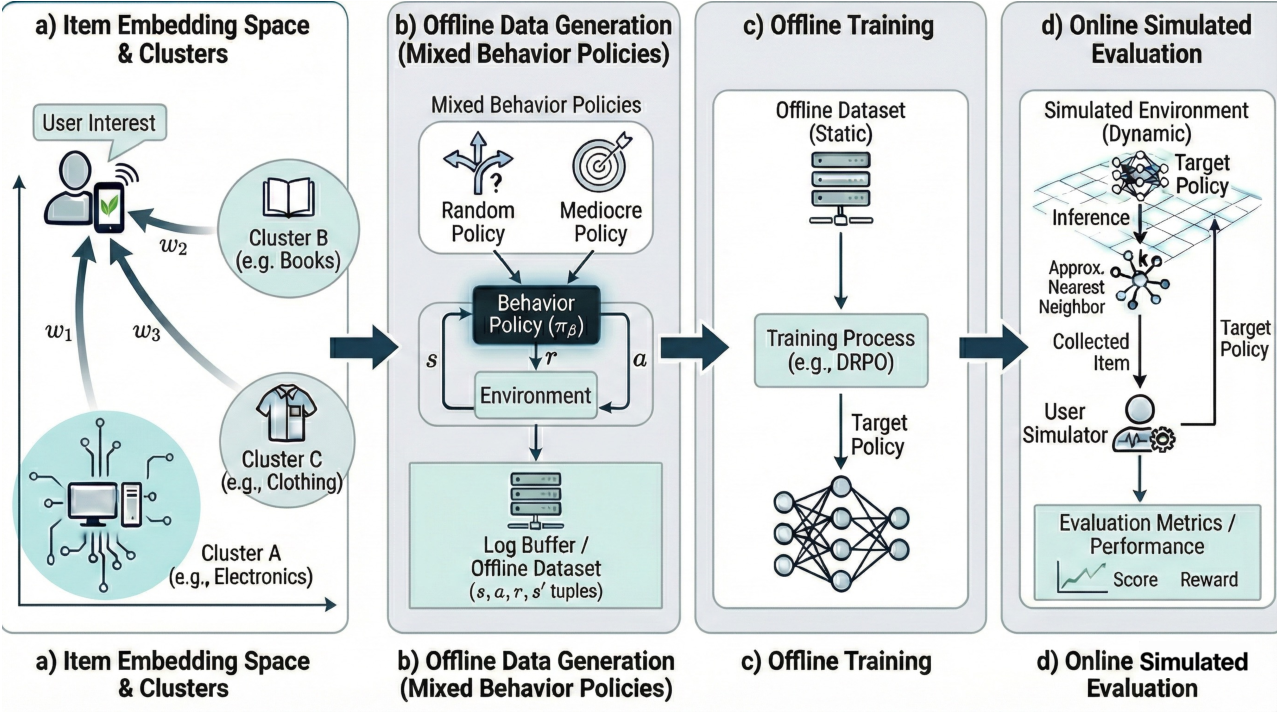
\includegraphics[width=0.95\linewidth]{figures/RecSim.pdf}
  \caption{Overview of RecSim. The system generates synthetic user-item interactions based on high-dimensional embedding clusters, featuring customizable noise injection and a mixed-strategy logging agent to replicate industrial data distributions.}
  \label{fig:sim_arch}
\end{figure}

\begin{figure}[htbp]
    \centering
    \begin{subfigure}[b]{0.48\textwidth}
        \centering
        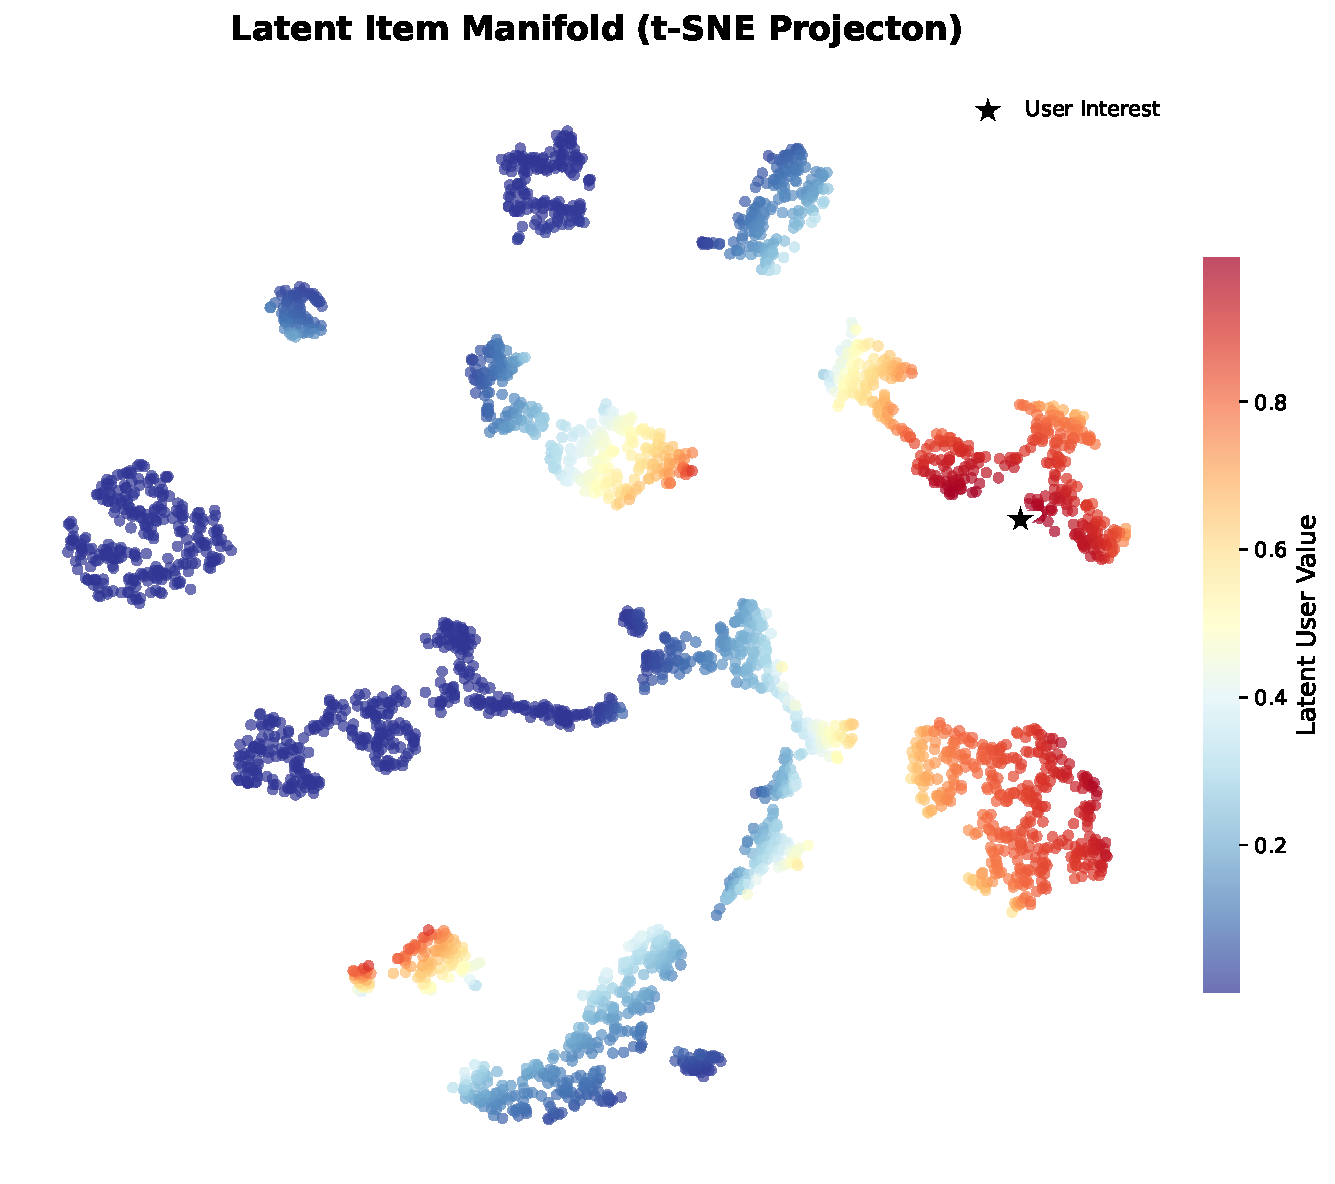
\includegraphics[width=\linewidth]{figures/visualization_tsne_academic.pdf}
        \caption{Latent Item Manifold (t-SNE Visualization)}
        \label{fig:recsim_viz_tsne}
    \end{subfigure}
    \hfill
    \begin{subfigure}[b]{0.48\textwidth}
        \centering
        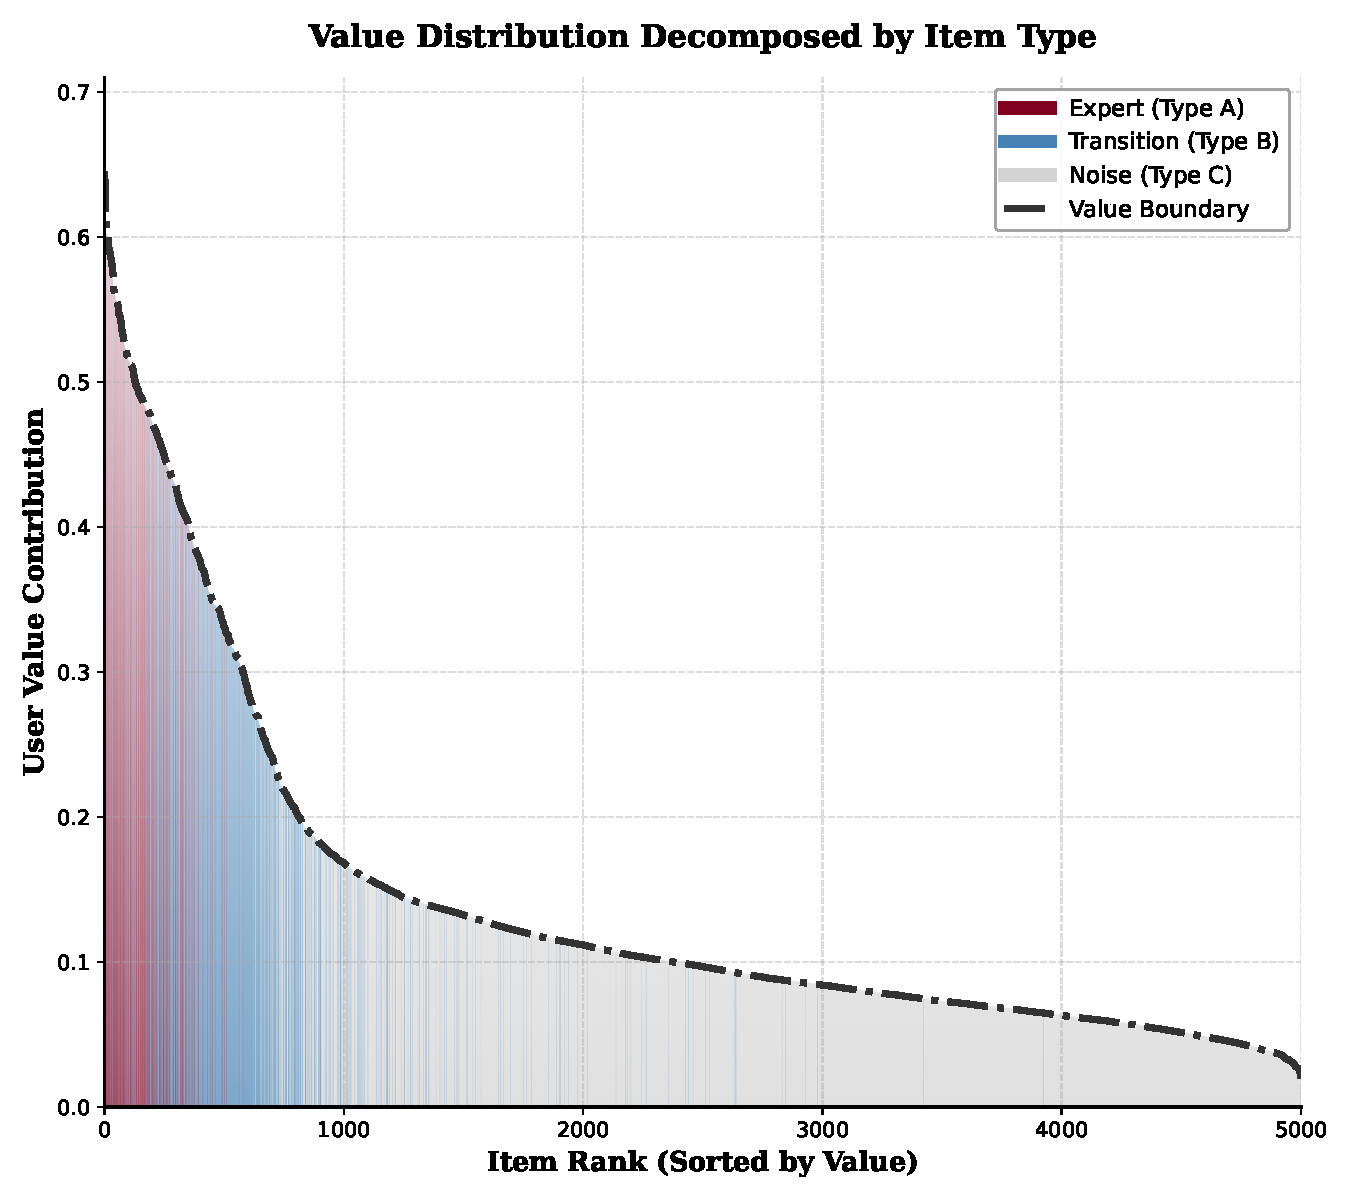
\includegraphics[width=\linewidth]{figures/visualization_reward_stacked.pdf}
        \caption{Value Distribution Decomposed by Item Type}
        \label{fig:recsim_viz_reward}
    \end{subfigure}
    \caption{Visualization of the RecSim Environment. (a) Visualization of the item space and user interest. For this plot, we set the simulation dimension to $d=3$ and utilize t-SNE to illustrate the relative spatial relationships between the User Interest (Star) and different item clusters. (b) The resulting power-law distribution of user values, decomposed by item types (Expert, Transition, Noise), highlighting the scarcity of high-value samples.}
    \label{fig:recsim_viz}
\end{figure}

\subsection{Embedding Topology and Retrieval}
\textbf{High-Dimensional Manifold.}
Standard datasets often treat items as independent discrete tokens. In contrast, RecSim models the item pool $\mathcal{I}$ and users $\mathcal{U}$ in a continuous embedding space $\mathbb{R}^d$. While the dimension $d$ is highly customizable to mimic various system architectures, we adopt the common industrial paradigm of $d=128$. This continuous representation ensures that the ``distance'' between items carries semantic meaning.
To intuitively demonstrate this topological structure, we specifically configured the simulation dimension to $d=3$ for the visualization experiment shown in Figure~\ref{fig:recsim_viz}(a), utilizing t-SNE to reveal the cluster distributions. The item distribution is generated via a Mixture of Gaussians (MoG) to simulate distinct latent topics (e.g., Cluster A vs. Cluster B). To further ensure fidelity, RecSim also supports initialization with real industrial embeddings. This topology enables us to implement KNN-based Retrieval for policy evaluation, strictly aligning with industrial vector search standards.

\textbf{User Value Function.}
The ground-truth user satisfaction is modeled as a function of geometric alignment in this space. We employ a radial basis function (RBF) centered on the user's latent interest $\mathbf{u}^*$, ensuring that the reward landscape is smooth and differentiable:
\begin{equation}
    R_{\text{latent}}(s, a) = \exp\left( - \frac{1 - \text{cos}(\mathbf{e}_a, \mathbf{u}^*)}{2 \delta^2} \right)
\end{equation}
This physics-based mechanism captures the high-dimensional correlation between user interests and item properties. The hyperparameter $\delta$ allows us to simulate diverse scenarios by adjusting the sensitivity of user preferences.

\subsection{Reproducing the Data Curse via Customizability}

A critical characteristic of online logs is the dominance of low-quality interactions. RecSim reproduces this \textbf{Data Curse} by deploying a Mixed Strategy Logging Agent. As visualized in Figure~\ref{fig:recsim_viz}(a), the spatial distribution of logged data reflects the entropy of real traffic:
\begin{itemize}
    \item \textbf{Noise Domination (Blue Points, $\pi_{\text{rand}}$):} Simulating cold-start phases or insufficient model capabilities, these interactions are effectively random. They account for a large portion of the logs but have extremely low relevance.
    \item \textbf{Bias Injection (Orange/Yellow Points, $\pi_{\text{pop}}$):} Representing popularity-based strategies. These items are recommended in high volumes but possess only moderate relevance to the specific user.
    \item \textbf{Signal Scarcity (Black Star, $\pi_{\text{expert}}$):} Representing items highly matched with user interest. These are located near the User Interest centroid but are extremely sparse.
\end{itemize}

Crucially, the aggregate item frequency in the generated logs adheres to a Zipfian distribution, faithfully replicating the severe popularity bias and long-tail characteristics ubiquitous in production environments. This mixture results in a Power-Law Reward Distribution, as shown in Figure~\ref{fig:recsim_viz}(b). High-quality samples (Expert, dark red region) occupy only the thin tail, while the vast majority of data (Noise/Transition) yields low rewards. By adjusting the mixture weights, we can customize the dataset to rigorously test DRPO's ability to reject noise (``trash'') and clone sparse expert signals.

\subsection{Aleatoric Uncertainty}
Finally, to mimic the stochastic nature of user feedback (e.g., accidental clicks), the observed reward stored in the logs is a corrupted version of the latent value:
\begin{equation}
    R_{\text{obs}} = \text{clip}\left( R_{\text{latent}} + \mathcal{N}(0, \sigma_{\text{noise}}^2), 0, 1 \right)
\end{equation}
Here, $\sigma_{\text{noise}}$ represents the inherent system noise. This forces the learner to differentiate between the true embedding structure (Signal) and the feedback randomness (Noise).

\subsection{Industrial Scenario Instantiation}
\label{app:scenario_mapping}

Leveraging the customizable components described above, we instantiated two distinct datasets to bridge the gap between offline simulation and real-world deployment stages. The configurations map directly to the \textbf{Ranking} and \textbf{Generative Retrieval} stages in industrial pipelines.

\paragraph{Scenario 1: Medium Quality (Impression-Click Feedback).}
This setting simulates the \textbf{Online Post-Exposure Logs}, corresponding to the real-world interactions collected after the retrieval and ranking phases.
\begin{itemize}
    \item \textbf{Industrial Logic:} Unlike the full corpus, this data consists only of items that were successfully \textbf{impressed} (exposed) to users and their subsequent \textbf{clicks}. Since these items have already passed the system's filtering funnel, the data quality is "Medium"—it contains valid interest signals but is heavily skewed by \textbf{Exposure Bias} (i.e., we only observe feedback on displayed items).
    \item \textbf{Configuration:} We construct this by mixing trajectories from a competent policy (simulating the exposure mechanism) with user feedback. The distribution reflects the \textbf{Impression Space} rather than the full Action Space.
    \item \textbf{Implication:} This mirrors the standard training environment for ranking models, where the goal is to learn from biased, semi-optimal exposure logs.
\end{itemize}

\paragraph{Scenario 2: Extreme Noisy (Generative Retrieval Stage).}
This setting simulates the \textbf{Full-Corpus Exploration Phase}, akin to Generative Retrieval \cite{rajput2023recommender}.
\begin{itemize}
    \item \textbf{Industrial Logic:} The model faces the entire action space. To ensure catalog coverage and solve the cold-start problem, the data collection policy must employ aggressive random exploration ($\pi_{\text{rand}}$).
    \item \textbf{Configuration:} We configure the logging agent to be noise-dominated, with $\pi_{\text{rand}}$ accounting for $90\%$ of the interactions.
    \item \textbf{Implication:} This creates a "needle in a haystack" problem. It serves as the ultimate stress test for robustness, evaluating whether DRPO can clone the sparse expert signal while rejecting the overwhelming heavy-tailed noise.
\end{itemize}

\begin{table}[h]
\centering
\caption{Configuration of Data Scenarios in RecSim. The "Extreme Noisy" setting is dominated by random exploration, creating a severe signal-to-noise ratio challenge.}
\label{tab:scenario_config}
\begin{small}
\begin{tabular}{l|ccc}
\toprule
\textbf{Scenario} & \textbf{Expert Policy} & \textbf{Suboptimal Policy} & \textbf{Random Noise} \\
& (High Reward) & (Medium Reward) & (Low Reward) \\
\midrule
\textbf{Medium Quality} & 10\% & 60\% & 30\% \\
\textit{(Impression Logs)} & \textit{(Sparse Signal)} & \textit{(Bias Dominated)} & \textit{(Background Noise)} \\
\midrule
\textbf{Extreme Noisy} & 5\% & 5\% & \textbf{90\%} \\
\textit{(Full Retrieval)} & \textit{(Needle in Haystack)} & \textit{(Negligible)} & \textit{(Overwhelming)} \\
\bottomrule
\end{tabular}
\end{small}
\end{table}

\section{Baseline Implementation Details}
\label{app:baselines}

To ensure a fair comparison, all baselines were implemented using the same backbone network architecture (a 3-layer MLP with ReLU activations) as DRPO. We performed a grid search for the key hyperparameters of each baseline.

\begin{itemize}
    \item \textbf{APG (Advantage Policy Gradient):} Optimizes the policy by directly applying the policy gradient with estimated advantages on the offline dataset, omitting importance sampling corrections. This approach ignores the distribution shift between the learned policy and the behavior policy, leading to severe divergence in high-noise settings.

    \item \textbf{BC (Behavior Cloning):} Minimizes the negative log-likelihood of the actions in the dataset. This serves as the foundation for regularized methods.
    \item \textbf{CRR (Critic Regularized Regression):} Uses the critic's Q-value estimate to filter samples. We tuned the $\beta$ parameter in $\{0.5, 1.0, 5.0\}$.
    \item \textbf{BPPO (Behavior Proximal Policy Optimization):} Constrains the policy update within a trust region of the behavior policy. We tuned the clip ratio $\epsilon \in \{0.1, 0.2, 0.3\}$.
    \item \textbf{AWR (Advantage Weighted Regression):} Performs regression with weights $w \propto \exp(A/\beta)$. We tuned the temperature $\beta \in \{0.05, 0.1, 1.0\}$.
    \item \textbf{IQL (Implicit Q-Learning):} Uses expectile regression to estimate values without querying out-of-distribution actions. We tuned the expectile $\tau \in \{0.5, 0.7, 0.9\}$.
    \item \textbf{AsymRe:} Applies fixed asymmetric weights to down-weight negative advantages. We used the standard configuration with down-weight factor $w^- = 0.1$.
    \item \textbf{Adaptive BC:} A strong ablation baseline that combines our proposed \textit{Variance-Guided Filtering} with standard Behavior Cloning. It trains strictly on the high-quality data subset selected by the adaptive filter, optimizing the negative log-likelihood without additional importance weighting. This baseline isolates the contribution of the filtering mechanism from the policy optimization objective. The filtering hyperparameters were kept identical to those in DRPO.
\end{itemize}

\section{Implementation Details and Hyperparameters}
\label{app:hyperparams}

In this section, we provide the detailed experimental setup and hyperparameter configurations for our proposed method, \textbf{DRPO} (Variance-Guided Filtering + AsymRe), and its variant \textbf{DRPO-exp} (Variance-Guided Filtering + AWR).

\subsection{Network Architecture}
All experiments are conducted in the End-to-End Recommendation System environment described in Section~\ref{sec:experiments}. \textbf{Following common industry practice, we formulate the recommendation problem as a Contextual Bandit task}, focusing on optimizing immediate rewards based on user contexts.


Given that our environment operates on \textbf{dense latent state representations} ($d=10$) , we employ a compact yet expressive architecture. Specifically, the policy network $\pi_\theta$ is parameterized as a Gaussian distribution where the mean is output by a 2-layer Multi-Layer Perceptron (MLP) with a hidden dimension of 128 and ReLU activations. This architecture effectively captures the non-linear relationships in the dense manifold without the computational overhead of large-scale embedding tables. The Value/Q networks used in baseline methods share the same backbone architecture.

\subsection{Hyperparameter Settings}
Table~\ref{tab:hyperparameters} lists the specific hyperparameters used. The \textit{Target Ratio} ($\rho$) is the core parameter of our Variance-Guided mechanism, controlling the strictness of the filtration. For DRPO-exp, the temperature parameter $\beta$ controls the sharpness of the advantage weighting.

\begin{table}[h]
    \centering
    \caption{Hyperparameter settings for DRPO and DRPO-exp.}
    \label{tab:hyperparameters}
    \vspace{2mm}
    \begin{tabular}{l|c|c}
        \toprule
        \textbf{Hyperparameter} & \textbf{Symbol} & \textbf{Value} \\
        \midrule
        \multicolumn{3}{l}{\textit{General Optimization}} \\
        \midrule
        Learning Rate & $\eta$ & $3 \times 10^{-4}$ \\
        Batch Size (Sampling) & $B_{\text{sample}}$ & 320 \\
        Optimizer & - & Adam \\
        Total Training Steps & $T$ & 5000 \\
        \midrule
        \multicolumn{3}{l}{\textit{Variance-Guided Filtering (Shared)}} \\
        \midrule
        Target Variance Ratio & $\rho$ & 0.5 \\
        Initial Top-P & $p_0$ & 0.5 \\
        Top-P Update Rate (Relax) & $\gamma_{\text{up}}$ & 1.02 \\
        Top-P Update Rate (Tighten) & $\gamma_{\text{down}}$ & 0.98 \\
        \midrule
        \multicolumn{3}{l}{\textit{Algorithm Specifics}} \\
        \midrule
        \textbf{DRPO} (Ours) & Objective & AsymRe \\
        & Baseline & $\min(R_{\text{subset}})$ \\
        \midrule
        \textbf{DRPO-Exp} (Variant) & Objective & AWR \\
        & Temperature $\beta$ & 0.05 \\
        & Baseline & $\text{mean}(R_{\text{subset}})$ \\
        \bottomrule
    \end{tabular}
\end{table}

\section{Extended Analysis on Noise Sensitivity}
\label{app:sensitivity}

In this section, we provide a detailed sensitivity analysis of the filtering threshold (Target Ratio) under various environmental conditions. This analysis serves as the empirical motivation for our proposed Adaptive Mechanism.

\begin{table}[h]
\centering
\caption{\textbf{Sensitivity Analysis: The Interplay of Reward and Policy Noise.}
We compare the performance (eCPM) of fixed target ratios under varying noise conditions.
\textbf{(1) Reward Noise Impact:} Low reward noise favors aggressive filtering (Top 5\%), while high reward noise requires conservative strategies (100\%) to avoid overfitting.
\textbf{(2) Policy Noise Impact:} When data quality degrades (Policy Noise $0.1 \to 0.5$), the unfiltered baseline (Ratio 100\%) suffers a severe performance drop ($1.20 \to 1.04$ in Medium Reward Noise), whereas filtering maintains robust performance.}
\label{tab:sensitivity_sweep}
\resizebox{\textwidth}{!}{
\begin{tabular}{l|ccc|ccc}
\toprule
\multirow{2}{*}{\textbf{Reward Noise}} & \multicolumn{3}{c|}{\textbf{Policy Noise = 0.1 (High Quality Data)}} & \multicolumn{3}{c}{\textbf{Policy Noise = 0.5 (Low Quality Data)}} \\
\cmidrule(lr){2-4} \cmidrule(lr){5-7}
 & Top 5\% & Top 40\% & 100\% (No Filter) & Top 5\% & Top 40\% & 100\% (No Filter) \\
\midrule
\textbf{Low (0.0)}   & \textbf{1.69} & \textbf{1.69} & 1.35 & \textbf{1.63} & \textbf{1.63} & 1.59 \\
\textbf{Medium (0.5)}& \textbf{1.29} & \textbf{1.29} & 1.20 & \textbf{1.13} & \textbf{1.13} & 1.04 \\
\textbf{High (1.0)}  & 1.06 & 1.06 & \textbf{1.13} & 0.87 & 0.87 & \textbf{0.93} \\
\bottomrule
\end{tabular}
}
\end{table}

\paragraph{Detailed Analysis.}
Table~\ref{tab:sensitivity_sweep} presents a comprehensive sweep of filtering thresholds across different noise regimes. We highlight two key observations:

\begin{itemize}
    \item \textbf{Robustness to Policy Degradation:}
    Comparing the two major columns, we observe that as data quality deteriorates (Policy Noise increases from $0.1$ to $0.5$), the performance of the unfiltered baseline (Ratio 100\%) drops significantly.
    For instance, under Medium Reward Noise, the baseline performance falls from $1.20$ to $1.04$.
    In contrast, aggressive filtering (Top 5\%-40\%) effectively mitigates this degradation, maintaining a higher performance floor.
    This confirms that when the behavior policy is suboptimal, identifying and cloning only the sparse high-quality signals is far more effective than imitating the entire distribution.

    \item \textbf{The "Overfitting to Noise" Dilemma:}
    Under High Reward Noise ($\sigma=1.0$), the trend reverses. Aggressive filtering (Top 5\%) yields suboptimal results ($0.87$) compared to the unfiltered baseline ($0.93$).
    In this regime, extremely high rewards are often driven by stochastic noise rather than true expertise.
    Filtering for these "outliers" causes the model to \textit{overfit to noise}, whereas retaining more data helps average out the zero-mean reward noise.
\end{itemize}

\paragraph{Conclusion.}
These conflicting requirements---filtering aggressively for bad policies but conservatively for noisy rewards---render any fixed hyperparameter suboptimal. This necessitates the proposed \textbf{Adaptive Mechanism}, which dynamically adjusts the filtering threshold to balance signal extraction against noise overfitting.

\end{document}
